%% LyX 2.4.2.1 created this file.  For more info, see https://www.lyx.org/.
%% Do not edit unless you really know what you are doing.
\documentclass[american,british,english]{article}
\PassOptionsToPackage{natbib=true}{biblatex}
\usepackage[LGR,T1]{fontenc}
\usepackage[utf8]{inputenc}
\pagestyle{plain}
\usepackage{color}
\definecolor{note_fontcolor}{rgb}{0.800781, 0.800781, 0.800781}
\usepackage{verbatim}
\usepackage{url}
\usepackage{varwidth}
\usepackage{amsmath}
\usepackage{amssymb}
\usepackage{graphicx}
\usepackage{geometry}
\geometry{verbose,tmargin=3cm,bmargin=3cm,lmargin=3cm,rmargin=3cm}
\usepackage{setspace}
\doublespacing
\usepackage{lineno}
\linenumbers

\makeatletter

%%%%%%%%%%%%%%%%%%%%%%%%%%%%%% LyX specific LaTeX commands.
\DeclareRobustCommand{\greektext}{%
  \fontencoding{LGR}\selectfont\def\encodingdefault{LGR}}
\DeclareRobustCommand{\textgreek}[1]{\leavevmode{\greektext #1}}

%% Because html converters don't know tabularnewline
\providecommand{\tabularnewline}{\\}
%% Variable width box for table cells
\newenvironment{cellvarwidth}[1][t]
    {\begin{varwidth}[#1]{\linewidth}}
    {\@finalstrut\@arstrutbox\end{varwidth}}
%% The greyedout annotation environment
\newenvironment{lyxgreyedout}
{\normalfont\normalsize\textcolor{note_fontcolor}\bgroup\ignorespaces}
{\ignorespacesafterend\egroup}

%%%%%%%%%%%%%%%%%%%%%%%%%%%%%% Textclass specific LaTeX commands.
\newcommand{\lyxaddress}[1]{
	\par {\raggedright #1
	\vspace{1.4em}
	\noindent\par}
}

%%%%%%%%%%%%%%%%%%%%%%%%%%%%%% User specified LaTeX commands.

% specify here the journal
%\journal{Methods in Ecology and Evolution}
% use this if you need line numbers
%\usepackage{lineno}  %%% PROBABLY DON'T in LyX 2.4 where line nums are easier
%\linenumbers
\usepackage{tikz}
\usetikzlibrary{arrows,automata,positioning,arrows.meta}
\usepackage[utf8]{inputenc}
\DeclareUnicodeCharacter{202A}{!!!FIX ME!!!}
\DeclareUnicodeCharacter{202C}{!!!FIX ME!!!}

% get rid of the note field (which has an eprint URL for most entries)
%\AtEveryBibitem{\clearfield{note}\clearfield{addendum}}
%\AtEveryCitekey{\clearfield{note}\clearfield{addendum}}
%\DeclareFieldFormat*{note}{}

\makeatother

\usepackage{babel}
\usepackage[style=authoryear,doi=false, isbn=false, maxcitenames=2, mincitenames=1,uniquelist=false, url=false, date=year, giveninits=true, eprint=false]{biblatex}
\addbibresource{walrusbib.bib}
\begin{document}
\title{Combining individual and close-kin mark-recapture to design an effective
survey for Pacific walrus }
\author{Eiren K. Jacobson\textsuperscript{1}\textsuperscript{{*}}, Mark
V. Bravington\textsuperscript{2}, Rebecca L. Taylor\textsuperscript{3},
\\
Irina S. Trukhanova\textsuperscript{4,5}, David L. Miller\textsuperscript{6},
William S. Beatty\textsuperscript{3,7}}
\maketitle

\lyxaddress{\textsuperscript{1} Centre for Research into Ecological \& Environmental
Modelling and School of Mathematics \& Statistics, University of St
Andrews, St Andrews, Scotland }

\lyxaddress{\textsuperscript{2} Estimark Research, Hobart, Australia}

\lyxaddress{\textsuperscript{3} US Geological Survey, Alaska Science Center,
Anchorage, Alaska}

\lyxaddress{\textsuperscript{4} North Pacific Wildlife Consulting, LLC, Seattle,
Washington}

\lyxaddress{\textsuperscript{5} US Fish and Wildlife Service, Marine Mammals
Management, Anchorage, Alaska}

\lyxaddress{\textsuperscript{6} 165 Perth Road, Dundee, Scotland}

\lyxaddress{\textsuperscript{7} US Geological Survey, Upper Midwest Environmental
Sciences Center, La Crosse, Wisconsin }

\lyxaddress{\textsuperscript{{*}}Corresponding author email: ej45@st-andrews.ac.uk}

\pagebreak{}

\subsection*{Acknowledgments}

\subsection*{Data availability}

\subsection*{Conflict of Interest statement}

\subsection*{Author contribution statements}

\subsection*{Statement on inclusion (optional)}

\pagebreak{}
\begin{abstract}
The Pacific walrus \emph{(Odobenus rosmarus divergens) }is an ice-associated
marine mammal found in the Bering and Chukchi Seas, where they have
been hunted for subsistence for time immemorial. In the late 20th
century, the population declined, likely because it had reached carrying
capacity and was subject to high harvests. Currently, Pacific walrus
is species of conservation concern due to the potential impacts of
climate change, particularly related to loss of sea ice. To reduce
uncertainty in estimates of population size and trend, researchers
undertook an individual genetic mark-recapture (IMR) sampling campaign
from 2013-2017 and collected tissue samples from over 8,000 individuals.
Another campaign of a similar scale is ongoing (2023-2027). While
sample collection was designed for IMR, advances in close-kin mark-recapture
(CKMR) methodology and associated molecular techniques mean these
samples could also be suitable for CKMR. The advantages of CKMR over
IMR include increased effective sample size (since each individual
tags not only itself, but also its parents, siblings, and offspring)
and additional insights into demographic quantities of interest. Here,
we combine individual and close-kin mark-recapture in a single modelling
framework (ICKMR) and investigate whether different sampling strategies
can increase precision in estimates of abundance and trend. Our modelling
approach includes special considerations for walrus life-history,
including a multi-year inter-birth interval. We implement our model
in R and use an individual-based simulation to test performance of
the ICKMR model. Something here about survey design. We find that
the expected precision of the ICKMR estimates of abundance are higher
than those expected from IMR alone. This result suggests that ICKMR
is a promising approach for assessing population size and trend of
species which have been difficult to survey using more traditional
methods. {[}285/350{]}
\end{abstract}
Keywords: Close-kin mark-recapture, individual genetic mark-recapture,
survey design, walrus  

\newpage{}

\section{Introduction\label{sec:Introduction}}

\selectlanguage{american}%

Estimation of abundance and of other demographic parameters such as
survival is a key part of wildlife management and conservation. Traditional
mark-recapture analysis \citep{williams_analysis_2002} can deliver
estimates with low bias and uncertainty, provided that enough individual
animals i) are naturally, artificially, or genetically “marked” and
identifiable and ii) can be recaptured over time. If genotypes are
used as the marks, as in genetic individual mark-recapture (IMR; \citealp{palsboll_genetic_1997}),
then kinship patterns amongst the samples (parents, siblings, etc)
contains additional information relevant to demographics \citep{skaug_allele-sharing_2001}.
Close-kin mark-recapture (CKMR; see \citealp{bravington_close-kin_2016})
is a framework for using these kinships, as inferred from genotypes,
to estimate abundance and demographic parameters. CKMR provides additional
flexibility compared with IMR since lethal samples (from sampling,
hunting, natural mortality etc.) and/or non-lethal samples can be
used; it also increases the effective sample size, since more types
of ``recapture'' are possible. As of 2025, most CKMR projects have
been for commercial fish (e.g., \citealp{Davies2020SBT2}) or sharks
(e.g., \citealp{Hillary2018WS-CKMR}), but there are also some for
mammals, including \citet{conn_robustness_2020}'s modeling study
of bearded seals and its implementation by \citet{taras_estimating_2024},
and \citet{lloyd-jones_close-kin_2023} for flying foxes.

The principle behind CKMR is that every individual has (or had) one
mother and one father; thus, for a given sample size, in a large population
there will be few ``recaptures'' of parents or their other descendants,
while in a small population there will be many. In practice, the data
for CKMR comprise the outcome of pairwise kinship checks amongst samples,
plus covariates associated with each sample such as its date of capture,
age, size, sex etc. The CKMR model has two components: a population-dynamics
part driven by the demographic parameters; and formulae for the expected
frequencies of different kinship types in pairwise comparisons, conditional
on sample covariates and population dynamics. By combining the kinship
data with the model, parameters can be estimated using maximum-likelihood
or Bayesian methods.

CKMR has mostly been used in situations where self-recaptures are
unlikely or impossible (e.g., because sampling is lethal). \citet{lloyd-jones_close-kin_2023}
did include IMR results in a CKMR study but did not integrate both
datasets into a single model. Here, we focus on a population where
IMR was the original project goal; therefore we extend traditional
CKMR to include IMR in the same model as an additional kinship type,
whereby pairwise genetic comparison can show that two samples are
from the same animal.

The success of CKMR and/or IMR depends on whether data collected contain
sufficient recaptures. Sampling design (e.g. number of samples, composition,
study duration, type and quality of covariate measurements) is crucial
to avoid expensive, embarrassing, and predictable failure. The pairwise-comparison
framework leads to analytical results for expected number of kin-pairs
and expected variance given expected number of samples (and associated
covariates), so that simulation is not essential; nevertheless, simulation
can be useful as a way to check the fairly complex code of kinship
probabilities and design setup. In this paper we show how to do and
check the calculations using a case study on the Pacific walrus (\emph{Odobenus
rosmarus divergens}; hereafter, walrus) in the North Pacific. We explore
different demographic and design scenarios for walrus using IMR alone
versus CKMR + IMR = ICKMR, and demonstrate how the latter can be used
to substantially reduce the overall amount of survey effort required
for adequate monitoring.

In the rest of this Introduction, we provide some background on CKMR
(drawn from \citealt{bravington_close-kin_2016} and experience on
projects since), and on walrus biology and the survey setup. In Methods,
we describe our walrus population dynamics model, derive walrus-appropriate
kinship probability formulae, and show how to analytically calculate
the expected variances that might come from different survey designs.
We also outline the simulation setup which we used to test our ICKMR
model. The Results section shows how different survey designs are
likely to perform (e.g., with\slash without CKMR). In the Discussion,
we summarize our conclusions for walrus, and also mention some modeling
simplifications made for design purposes that we may wish to reconsider
when working with real data.

\subsection{Walrus biology and background}

The walrus is a gregarious, ice-associated pinniped inhabiting continental
shelf waters of the Bering and Chukchi seas. During winter (when sea
ice forms south of the Bering Strait) virtually all walruses occupy
the Bering Sea \citep{fay_ecology_1982}. In summer (when sea ice
is absent from the Bering Sea) almost all juvenile and adult female
walruses, and some adult male walruses, migrate north to the Chukchi
Sea. When walruses rest offshore on sea ice floes, their distribution
is dynamic, because it generally follows the marginal ice zone (a
moving, changing habitat which contains a mix of ice floes and water)
but also concentrates in regions of high benthic productivity. This
allows walruses to forage for benthic invertebrates while simultaneously
having access to a nearby substrate for hauling out.

{*}{*}{*}NEED something about walrus moving about all over the place,
from IMR data and (more likely) sat tags :) Some of that {*}could{*}
go to the Discussion, but I think at least a pre-mention here, coz
it will otherwise be in the alert reader's mind as they look at the
model structure

{*}{*}{*}Walrus reprod biol summary could go here? Rather than putting
it off until Methods. See sec 2.1

Sea ice has declined for decades \citep{perovich_loss_2009,stroeve_trends_2012,stroeve_changing_2018},
and coupled global atmospheric-ocean general circulation models predict
its continued decline \citep{arthun_seasonal_2021}. When sea ice
recedes from the continental shelf, walruses come on shore to rest
in large herds at sites termed haulouts, from which they make long
trips to foraging hotspots \citep{jay_walrus_2012}. This change in
their activity budgets \citep{jay_walrus_2017} may ultimately lead
to a decline in body condition and an increase in mortality or a decrease
in reproduction \citep{udevitz_forecasting_2017}. Furthermore, disturbance
at haulouts can cause stampedes, resulting in mass calf and juvenile
mortality. Continued sea-ice loss and a concomitant increase in the
intensity and expansion of industrial and shipping activities in Pacific
Arctic waters \citep{silber_vessel_2019} are expected to drive a
substantial population decline \citep{garlich-miller_status_2011,maccracken_final_2017,johnson_assessing_2023,johnson_assessing_2024}.

Range-wide abundance and demographic rate estimates are crucial for
understanding population status, as well as for developing and implementing
harvest management plans. In particular, subsistence walrus harvests
in Alaska and Chukotka exceed 4,000 animals annually (USFWS, 2023),
and indigenous peoples need information on the status of the walrus
population in order to manage these harvests sustainably. Furthermore,
in the United States, the Marine Mammal Protection Act (MMPA) requires
a determination of potential biological removal for walrus, which
in turn, requires a precise abundance estimate \citep{gilbert_review_1999,wade_determining_1999}.

Scientists have attempted to ascertain walrus population size since
at least 1880 \citep{fay_managing_1989}, and until very recently,
unsuccessfully. The most concerted effort was the 1975-2006 range-wide
airplane-based surveys conducted collaboratively with the Soviet Union
and then Russian Federation. However, resulting estimates were biased
and imprecise, and count-based methods were abandoned after the 2006
survey which, despite a rigorous design, innovative field methods,
and sophisticated analyses, yielded a 95\% confidence interval (CI)
on the population size estimate of 55,000–507,000 animals (CV = 0.93).
The extensive imprecision in the estimate resulted from the walrus
population being widely dispersed with unpredictable local clumping
\citep{speckman_results_2011,jay_walrus_2012}, which is, in turn,
due to the large area of arctic and subarctic continental shelf over
which they forage, their gregarious nature, and the dynamic nature
of the marginal ice zone.

The first rigorous walrus survival rate estimates were obtained within
the past decade via Bayesian integrated population models (IPMs),
which combined multiple data sources to estimate demographic rates
and population trend over multiple decades \citep{taylor_demography_2015,taylor_demography_2018}.
However, the original problems with the aerial survey data continued
to preclude conclusions about population abundance in the IPMs \citep{taylor_demography_2015}.

In 2013, the U.S. Fish and Wildlife Service (FWS) initiated a genetic
IMR project to estimate walrus abundance and demographic rates. Under
this approach, genetic ``marking'' via skin biopsy samples \citep{palsboll_genetic_1997}
provided a major advantage over traditional marking techniques because
walruses are extremely difficult to handle physically. Over five years
of research cruises, biologists attempted to collect a representative
sample of walruses in the accessible portion of the marginal ice zone
in each year a cruise was conducted, although Russian waters were
not accessible in all years. Sampling focused on groups of adult females
and juveniles, as these classes are the demographically important
population segments of this polygynous species \citep{fay_ecology_1982}.
Further methods for the IMR study are detailed by Beatty et al. (\cite*{beatty_panmixia_2020,beatty_estimating_2022}).

Data analysis from the first generation of walrus research cruises
(2013–2017) used a Cormack-Jolly-Seber multievent model to estimate
survival rates, and a Horvitz-Thompson-like estimator to obtain population
size. The total abundance of 257,000 had a 95\% credible interval
(CrI) of 171,000–366,000 (CV=0.19; \citealt{beatty_estimating_2022}).
Although the precision of the abundance estimate from the IMR study
was much improved over the final aerial survey, the IMR study required
extensive investment of human and financial resources (i.e, USD \$5,000,000).
A more cost-effective approach is needed to assess the walrus population
on a regular interval. As mentioned above, biopsy samples also contain
information about kin relationships, which, through CKMR, can substantially
augment the information content of genetic IMR without increasing
sampling effort. {[}1526 words{]}.\selectlanguage{english}%



\section{Methods\label{sec:Methods}}

To evaluate our proposed survey designs, we must first construct our
ICKMR model for walrus. We encode our knowledge about walrus biology
and life history to (\textit{i}) build a model of walrus population
dynamics, including the breeding cycle, and (\textit{ii}) formulate
kinship probabilities between pairs of samples. The population dynamics
model incorporates demographic parameters that will need to be estimated:
survival rates, adult abundance in some reference year, trend, and
so on. The kinship probabilities depend on the population dynamics.
Given a real dataset, we would estimate the parameters by maximizing
the log-likelihood that combines the kinship probabilities with the
actual outcomes of all pairwise comparisons. For design purposes,
though, we instead use a computational shortcut to predict the precision
of the estimates that would be expected under different sampling designs.
Although it is not strictly necessary to simulate any data in this
process, we did use simulations to check that our CKMR model was appropriately
formulated. This section describes our population dynamics model,
kinship probability formula, design calculations, and simulation setup.

\subsection{Biological considerations}

Adult males are inaccessible to this study given seasonal sex-segregation
and the geographical coverage of sampling effort (see Section \ref{sec:Introduction}).
They also form leks and compete for breeding access to females, so
it is plausible that adult males might also exhibit persistent individual
variability in breeding success, which would considerably complicate
the interpretation of paternal half-sibling kinship data (see Discussion).
Therefore, we restrict attention to female-only dynamics, and consider
only three types of kinship: Mother-Offspring Pair (MOP), Cross-cohort
maternal Half-Sibling Pair (XmHSP), and Self Pair (SP), i.e. recapture
of an individual. Our samples comprise juvenile and adult females,
plus juvenile males; the problems are with modelling males as parents,
but we can safely use sampled juvenile males as potential offspring
of females and as potential maternal half-siblings of other (female
or male) samples. We do not expect females to vary much in terms of
individual fecundity.

We assume that age estimates will be available for all samples, based
on epigenetic data (CITE). Visual classification is only accurate
over the first couple of years of life (CITE), which could be problematic
for CKMR. Our model is structured to allow for errors in estimated
age (with standard deviation assumed known i.e., after calibration
of epigenetic against known-age samples), though the results here
assume that there are no errors; see Discussion.

\subsubsection{Stage-structured quasi-equilibrium dynamics}

For our female-only population dynamics model, we opted for a stage-structured
(juvenile/adult), rather than fully-age-structured approach. We did
this because (\textit{i}) most female adults are expected to have
similar reproductive capacity and chance of survival, regardless of
age; and (\textit{ii}) stage-structured models are simpler to code
for CKMR and require fewer parameters (the addition of IMR data makes
things less simple). Stage-structured results should be quite adequate
for design purposes; the fundamental role of total (non-age-specific)
adult abundance and survival is very similar to fully-age-structured
models.

We used two stages: juveniles aged 1–5, and adults aged 6+ (the first
age at which an accompanying calf is common) at sampling. We did not
consider calves (age 0), to avoid complications around mother-calf
sampling. We assume constant survival within each stage ($\phi_{\text{A}}$
and $\phi_{\text{J}}$), and that offspring survival from age 1 onwards
is independent of its mother's survival, whether or not the offspring
has weaned yet. We assume that adult female abundance is stable, increasing,
or decreasing exponentially over the period covered by the population
dynamics (2000–2028; the lower limit of $y_{0}=$2000 is set because
there were fairly drastic changes in the population prior to that).
We have
\begin{align}
N_{y,\text{A}} & =N_{y_{0},\text{A}}e^{r(y-y_{0})}\label{popdyn}
\end{align}
where $N_{y,\text{A}}$ is the abundance of adult females in year
$y$, and $e^{r}$ is the rate of population increase.

Age composition within stage does not matter for MOP and XmHSP probabilities,
but is relevant for SPs. For that purpose, we assume that age composition
over the period is adequately described by the stable-age or ``quasi-equilibrium\textquotedbl{}
distribution consistent with survival $\phi_{\text{A}}$ and rate-of-increase
$e^{r}$. As shown in e.g., \citet{keyfitz2005applied} Chapter 5,
this is  $N_{y,a}\propto N_{y,\text{A}}\phi_{\text{A}}^{a}e^{-ra}$.

\subsubsection{The breeding cycle\label{subsec:The-breeding-cycle}}

We use a Markov model to describe the walrus breeding cycle. We assume
three breeding states: (S1) pregnant; (S2) with young-of-the-year
(YOTY) calf; or (S3) non-breeding, i.e., neither of the above. The
Markov property assumes that next year's state depends only on this
year's. From state S1 (pregnant), next year's state must be S2 (with
YOTY calf). From state S2, a female may next year either return to
state S1 (become pregnant again), with probability $\psi_{2}$, or
move to state S3 (neither pregnant nor with calf) with probability
$1-\psi_{2}$. From state S3, she will either move to state S1 (become
pregnant) with probability $\psi_{3}$, or remain in state S3 with
probability $1-\psi_{3}$. Due to long gestation times (\textasciitilde 14
months), walrus cannot give birth to calves in two consecutive years
(CITE). We also allow $\psi_{2}\neq\psi_{3}$ as they are unlikely
to give birth to calves every second year (CITE). This is shown in
Figure~\ref{fig:Breeding-cycle}. Survival is assumed to be independent
of breeding state. Females enter state S3 (i.e., reach sexual maturity)
on reaching age 4, and therefore can become pregnant at age 5 and
give birth at age 6. Depending on the values of $\psi_{2}$ and $\psi_{3}$,
this leads to a ramping-up in effective fecundity (i.e., probability
of being in state S2) over the first few years of adult life. Both
$\psi_{2}$ and $\psi_{3}$ are estimated from the data. We do not
use any data on whether females were with/without calf when sampled,
so the estimates of $\psi_{2}$ and $\psi_{3}$ are ultimately reliant
on the distribution of birth-gaps between maternal half-sibling pairs.

\begin{figure}
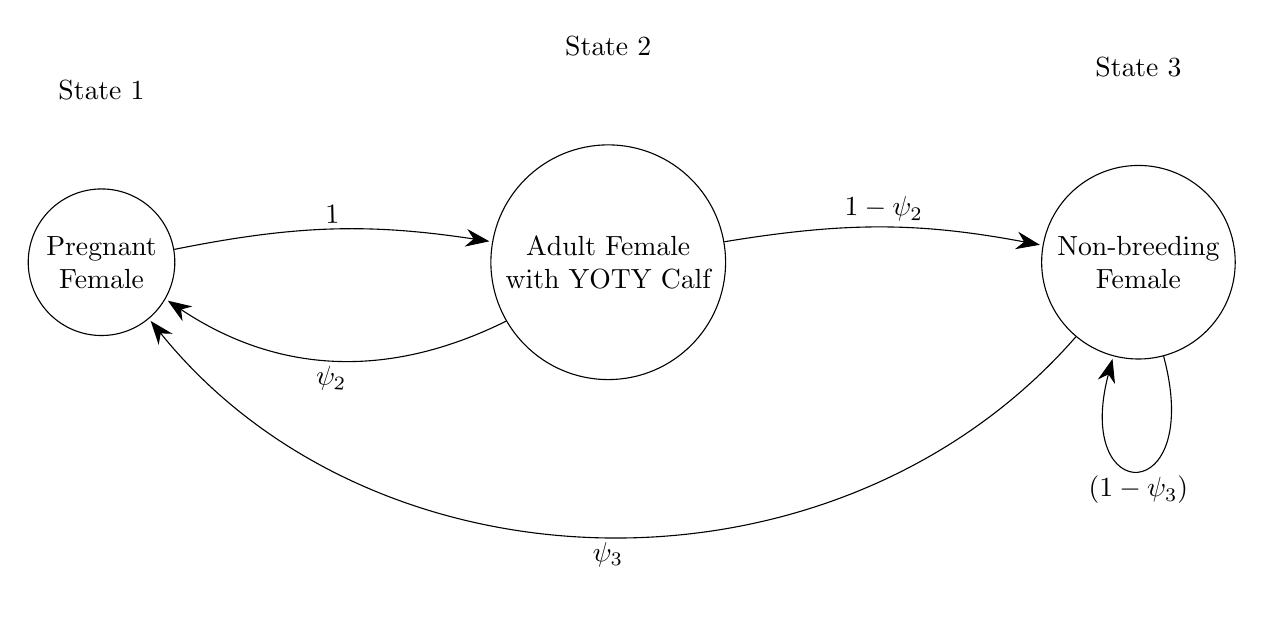
\begin{tikzpicture}[
    shorten > = 1pt,
node distance = 1cm and 4cm,
    el/.style = {inner sep=2pt, align=left, sloped}
                    ]

\node (q0) [state, align = center]             {Pregnant \\ Female};
\node (q1) [state,right=of q0, align = center] {Adult Female \\with YOTY Calf};
\node (q2) [state,right=of q1, align = center] {Non-breeding\\ Female};

\path[arrows=-{Stealth[length=3mm]}] 
    (q0)  edge [bend left=10]  node[el,above]  {$1$}         (q1)
    (q1)  edge [bend left=10]  node[el,above]  {$1-\psi_2$}         (q2)
    (q2)  edge [bend left=50]  node[el,below]  {$\psi_3$}         (q0)
    (q1)  edge [bend left=30]  node[el, below] {$\psi_2$}  (q0)

    ;

\draw[->,>= {Stealth[length=3mm]}]      (q2)  edge [loop below] node[el,below] {$(1-\psi_3)$}   (q2);

\node (e1)  [above=of q0] {State 1};
\node  (e2) [above=of q1] {State 2};
\node (e3) [above=of q2] {State 3};
\end{tikzpicture}

\caption{Directed cyclic graph showing the breeding cycle for walrus as represented
in our Markov model. Nodes in the graph show the states (pregnant,
with young-of-the-year (YOTY) calf, or non-breeding) and edges give
the probabilities of transition between those states. Walrus reach
sexual maturity at age 4, so females enter the graph at node non-breeding.
\label{fig:Breeding-cycle}}
\end{figure}

We will later use two quantities, which are derived from the breeding
cycle. First, we need to calculate the (average) proportion of adult
females in S2, $\bar{\beta}_{2}$. Let $\Psi$ be the (3$\times$3)
transition matrix implied by Figure~\ref{fig:Breeding-cycle}. Taking
the the eigendecomposition of $\Psi$, we can extract the second element
of the eigenvector with the largest eigenvalue to obtain $\bar{\beta}_{2}$.
We can then define fecundity as a function of age
\begin{gather}
F\left(a\right)\triangleq\frac{\mathbb{P}\left[B\left(a\right)=2\right]}{\bar{\beta}_{2}},\label{eq:fec-def}
\end{gather}
so that immature animals have fecundity 0, and an average adult has
fecundity 1.

\subsubsection{Formulating kinship probabilities}

We now need to formulate the demographic probabilities that two samples
have a given kinship, using the ERRO principle. We write the kinship
for individuals $i$ and $j$ as $K_{ij}$, which in our case may
be MOP, XmHSP, SP, or UP. In the case of MOPs and XmHSPs, we take
care to use only one sample from each individual (so ``sample''
and ``individual'' are interchangeable terms), whereas for SPs we
need to consider multiple samples from one individual (in which case,
``sample'' and ``individual'' have different meanings).

Throughout we use the following notation: for individual \emph{$i$},
sampled at age $a_{i}$ in year $y_{i}$ with birth year $b_{i}\triangleq y_{i}-a_{i}$.
As noted above, we only consider female abundance, so throughout $N$
refers to females only. When female abundance is considered for a
given year ($y$) and development stage ($d=\text{A}$ or $\text{J}$,
for adult or juvenile, respectively), it is written with two arguments,
$N_{y,d}$. We define the binary variable $L$ to indicate lethality
of sampling ($L_{i}=1$ indicating lethal sampling for individual
$i$). We use $\mathbb{I}()$ as an indicator function, giving 1 when
the condition inside the brackets is true, else 0. Kinship probabilities
are functions of demographic parameters such as $\phi_{\text{A}}$and
$N_{y_{0},\text{A}}$; we use $\boldsymbol{\theta}$ as shorthand
for this set of parameters, which become explicit in later iterations
of the formulae.

\subsubsection{Mother-offspring pairs (MOPs)}

Suppose we are about to compare a potential mother \emph{i}, to a
potential offspring \emph{j}. We restrict attention to comparisons
that satisfy the following:
\begin{itemize}
\item \emph{$i$} is female (though \emph{$j$} need not be);
\item $a_{j}\geqslant1$ (no calf samples are used);
\item $b_{j}\geqslant2000$ (population dynamics starts at year 2000).
\end{itemize}
We can now distinguish two cases: $y_{i}<b_{j}$ and $y_{i}\geqslant b_{j}$.

For $y_{i}<b_{j}$, individual \emph{i} still has to survive several
years in order to be individual \emph{j}'s mother (note that \emph{i}
may be immature when sampled, but mature by the time of \emph{j}'s
birth). In this case $i$'s sampling \textit{must} be non-lethal ($L_{i}=0$).
The MOP probability is
\[
\mathbb{P}\left[K_{ij}=\text{MOP}\vert a_{i},y_{i},b_{j},L_{i}=0,\boldsymbol{\theta}\right]=\frac{R_{i}(b_{j}\vert y_{i},a_{i})}{R^{+}(b_{j})}.
\]
where $R_{i}(b_{j}\vert y_{i},a_{i})$ is the expected reproductive
output (ERO) of individual $i$ in year $b_{j}$ given $i$ is age
$a_{i}$ in year $y_{i}$. $R^{+}(b_{j})$ is the total reproductive
output (TRO) of the whole population in year $b_{j}$. ERO and TRO
are in units of \textquotedbl number of calves\textquotedbl{} here
(though generally their units are arbitrary but matching). TRO is
the total number of adult females in the population when $j$ is born,
$N_{b_{j}\text{A}}$, multiplied by the proportion of females with
calves (breeding state S2), $\bar{\beta_{2}}$: $R^{+}(b_{j})=\bar{\beta_{2}}N_{b_{j},\text{A}}$.

There are two components to $i$'s ERO: first, she has to survive;
second, she has to be calving (breeding state 2) in $b_{j}$:
\[
R_{i}\left(b_{j}\vert y_{i},a_{i}\right)=\Phi\left(y_{i}-b_{j},a_{i}\right)\mathbb{P}\left[B\left(a_{i}+b_{j}-y_{i}\right)=2\right],
\]
where $\Phi\left(\Delta t,a\right)$ gives the probability of survival
for $\Delta t$ years, starting from age $a$ (product of annual juvenile
and adult survival probabilities). $B\left(a\right)$ is an individual's
breeding state in year $a$, which here is individual \emph{$i$}'s
age at $b_{j}$ ($a_{i}+b_{j}-y_{i}$, assuming she survives).

Then, using our definition of fecundity at age, \eqref{eq:fec-def},
we have
\begin{gather}
\mathbb{P}\left[K_{ij}=\text{MOP}\vert a_{i},y_{i},b_{j},L_{i}=0,y_{i}<b_{j},\boldsymbol{\theta}\right]=\frac{\Phi\left(y_{i}-b_{j},a_{i}\right)F\left(a_{i}+b_{j}-y_{i}\right)}{N_{b_{j},\text{A}}}.\label{eq:MOP-future}
\end{gather}

If \emph{$i$} is sampled after $j$'s birth ($b_{j}<y_{i}$). We
then know \emph{$i$} was alive (or not born yet), so there are no
lethality nor survival terms to worry about, but she may not have
been mature. Letting $F\left(a\leqslant0\right)=0$ (walruses cannot
breed before birth),
\begin{gather}
\mathbb{P}\left[K_{ij}=\text{MOP}\vert a_{i},y_{i},b_{j},b_{j}<y_{i},\boldsymbol{\theta}\right]=\frac{F\left(a_{i}-y_{i}-b_{j}\right)}{N_{b_{j},\text{A}}}.\label{eq:MOP-past}
\end{gather}


\subsubsection{Maternal half-sibling pairs (XmHSPs)}

We now find the probabilities of cross-cohort (X), maternal (m), half-sibling
pairs (HSP): XmHSPs. We want to compare individual \emph{$k$} to
individual \emph{$l$}, to check whether they have the same mother.
We restrict attention to comparisons that satisfy the following criteria:
\begin{itemize}
\item $b_{l}>b_{k}$ (avoiding double-counting);
\item $b_{k}\neq b_{l}$ (walrus give birth to a single offspring at a time);
\item $b_{k}\geqslant2000$ (population dynamics starts at 2000).
\end{itemize}
We know that $k$ definitely had a mother, whom we shall call $m$.
What is the probability that $l$'s mother was also $m$, given what
we know about $m$? The latter is that \textit{\emph{ }}\emph{$m$}
was alive, mature, and in breeding state S2 at $k$'s birth, andalso
\emph{$m$} survived at least one more year after\emph{ }$k$'s birth,
otherwise \emph{$k$} would not have lived long enough to be sampled.
In order for \emph{$m$} to be $l$'s mother, three more things have
to happen:
\begin{enumerate}
\item $m$ survives until $b_{l}$;
\item $m$ is in breeding state S2 in $b_{l}$;
\item amongst all the females that are alive and in the right breeding state
in year $b_{l}$, $m$ is the one who happens to be $l$'s mother.
\end{enumerate}
Let $\Phi\left(\Delta t\right)$ be the adult probability of survival
for $\Delta t$ years from \textquotedbl now\textquotedbl{} and recall
$\Psi$ is the breeding cycle transition matrix. The probability 3-vector
of an animal being in each state (S1, S2, S3) at time $t$ is $p^{\left[t\right]}$.
The probability vector at time $t+1$ is then $p^{\left[t+1\right]}=\Psi p^{\left[t\right]}$.
Now define $p^{\left[0\right]}=\left(0,1,0\right)^{\top}$which is
the probability vector of \emph{$m$}'s breeding state at $k$'s birth
(certain state 2), and recall $\bar{\beta}_{2}$ is the proportion
of adult females in breeding state S2. Then

\begin{gather}
\mathbb{P}\left[K_{k\ell}=\text{XmHSP}|b_{k},b_{\ell},\theta\right]\nonumber \\
=\mathbb{P}\left[K_{km}=\text{MOP}|B_{m}\left(b_{k}\right)=\text{S2},m\text{ alive at }b_{k}+1,b_{\ell},\theta\right]\nonumber \\
=\frac{\Phi\left(b_{l}-b_{k}-1\right)\left[\Psi^{b_{l}-b_{k}}p^{\left[0\right]}\right]_{2}}{N_{b_{l},\text{A}}\bar{\beta}_{2}}\label{eq:xmhsp}
\end{gather}

where $\left[\right]_{2}$ gives the second element of the vector,
i.e. the probability that \textit{m} (given she was alive) was again
in breeding state S2 at \textit{l}'s birth.

HSPs are just one of several ``second-order'' kin-pairs that are
practically indistinguishable genetically, hence cannot be identified
directly and unambiguously. Fortunately, HSPs are demographically
the most common when the birth-gap is short. When the birth-gap approaches
twice the age-of-maturity, though, GGPs (Grandparent-Grandchild Pair)
are more common. We deal with this by restricting the range of birth
gaps used in the model to those where GGPs are very rare (e.g., below
twice the age at maturity).

\subsubsection{Self-recaptures (SPs)\label{subsec:selfPs}}

Our stage-structured model keeps the population dynamics simple, but
we do have to make extra assumptions about sampling selectivity to
include the IMR data. Here, we assume that selectivity varies only
by stage (adult/juvenile), not by age within stage. We only consider
female samples for self-recapture, since juvenile males are prone
to \textquotedbl permanent emigration\textquotedbl{} (CITE) as well
as true mortality, so do not yield readily-interpretable inferences.

To compute stage-structured self-recapture probabilities, we condition
on the age of the first sample but \emph{not} explicitly on the age
of the second sample; instead we condition on the second sample's
developmental stage at sampling ($d_{2}$). If the first sample would
have reached the right developmental stage (otherwise, the two cannot
be the same animal), then we assume it is equally likely to be \emph{any}
of the females in that developmental stage at that year (i.e., sampling
is unselective within developmental stage) and thus the chance it
is the same as the second sample is the reciprocal of the developmental
stage abundance. We must also include survival for the intervening
years. The self-recapture kinship probability between samples 1 and
2 is (where $y_{1}<y_{2}$):

\begin{gather}
\mathbb{P}\left[K_{12}=\text{SP}\vert a_{1},y_{1},d_{2},y_{2},L_{1}=0,\boldsymbol{\theta}\right]=\frac{\mathbb{I}\left[d\left(a_{1}+\left(y_{2}-y_{1}\right)\right)=d_{2}\right]\Phi\left(y_{2}-y_{1},a_{1}\right)}{N_{y_{2},d_{2}}},\label{eq:self-staged}
\end{gather}
where $d\left(a\right)$ is the function that maps age to developmental
stage, with $d\left(a<6\right)=\text{"juvenile"}$ and $d\left(a\geqslant6\right)=\text{"adult"}$.
We also condition on the first sample being non-lethal (since we have
a second sample). To obtain $N_{y_{2},d_{2}}$, adult abundance is
part of the population dynamics model, but some more work is required
to deduce juvenile abundance. Assuming stable age composition, we
show in Appendix \ref{sec:Deriv-Njy} that for walrus:

\[
N_{y,\text{J}}=N_{y,\text{A}}\frac{\rho-\phi_{\text{A}}}{\rho-\phi_{\text{J}}}\left(\left(\frac{\rho}{\phi_{\text{J}}}\right)^{5}-1\right),
\]
where $\rho=e^{r}$ is the relative annual population increase/decrease.

A purely-age-structured version of \eqref{eq:self-staged} would need
to explicitly keep track of numbers-at-age, not just adult abundance
(as would the other kin types). The quasi-equilibrium assumption might
allow us to do this, but that assumption directly constrains relative
abundances-at-age. Thus, for example, the age 10 samples would then
provide direct estimates of the abundance of age 30 samples. In practice,
a fully age-structured CKMR formulation for walrus will need something
more sophisticated and time-varying than a quasi-equilibrium age distribution,
and therefore additional parameters to estimate. We therefore opted
for a stage- rather than age-structured SP model in the hope that
the overall statistical information content about total abundance
is reasonably realistic compared to what we might get from a more
complicated population dynamics model.

\subsection{Simulations}

We developed an individual-based simulation with the life history
and population dynamics of Pacific walrus to test our ICKMR model.
The simulation was modified from the R package \texttt{fishSim} by
Shane Baylis (\url{https://github.com/SMBaylis/fishSim}). The simulation
is stochastic and operates on an annual basis. Individuals are tracked
through the use of unique identifiers so that kinship pairs can be
identified in simulated samples. We initialized the simulation in
1950 with a population of 250,000 animals. These individuals are considered
``founders'' and do not have mothers or fathers. The age and sex
structure of the initial population is determined by the survival
rates used in the simulation (Table~\ref{tab:demo-pars}), which
were based on rates reported in \citet{taylor_demography_2018}. Individuals
that are at or beyond the age of first reproduction mate randomly
and males can potentially father more than one calf. Females reproduction
follows Section~\ref{subsec:The-breeding-cycle}. Females that are
in state 2 of the breeding cycle give birth to a single offspring
with 1:1 sex ratio. There is no systematic age-effect on female reproductive
dynamics, except that they are guaranteed not-pregnant in the year
immediately prior to maturity (Section~\ref{subsec:The-breeding-cycle}),
which slightly lowers effective fecundity for the first few years
of adulthood until the Markov chain reaches equilibrium. We did not
include senescence in our CKMR model, but we do include it in our
simulations. Parameters in Table~\ref{tab:demo-pars} were adjusted
to maintain the desired population rate of increase ($r$).

In sampling years, captures are simulated according to either historical
or planned future sample sizes. Females are available to be sampled
at any age, while only calf and juvenile males are available for sampling.
For simulated captures between 2014 and 2017, we used the realized
sample sizes by age or age class as the basis for simulation. For
simulated captures between 2023 and 2027, we used the target number
of samples per age class as the basis for simulation. After sampling,
some individuals die (according to age and/or sex specific mortality
rates, Table \ref{tab:demo-pars}). If a female with a young-of-the-year
calf dies, her calf also dies. Individuals automatically die if they
reach the maximum age. Living individuals then have their age incremented.

The female breeding cycle is as described in Section \ref{subsec:The-breeding-cycle}.
Although we assume in the simulation that all pregnancies result in
live births, this rate is aliased with the nominal calf-survival probability,
since only samples from age 1 onwards are considered; only the product
(nominal pregnancy success rate $\times$ nominal calf survival) affects
the simulated samples, not the two constituent parameters. Males and
females < 4 (or > the age of last reproduction; ALR) are exempt from
this cycle. The simulation then proceeds to the following year.

All simulations had a starting population size of 250,000 and were
run from 1950 to 2030. 

\begin{table}
\caption{Demographic parameters for simulation under four scenarios (D0, D1,
D2, and D3)\label{tab:demo-pars}}

\begin{tabular}{ccccc}
 & \multicolumn{4}{c}{Demographic Scenario}\tabularnewline
\cline{2-5}
 & D0 & D1 & D2 & D3\tabularnewline
Parameter & NULL & Stable & Decreasing & Increasing\tabularnewline
\hline 
Maximum age (AMAX) & 37 & 37 & 37 & 37\tabularnewline
Age at first reproduction for females (AFR) & 6 & 6 & 6 & 6\tabularnewline
Age of last reproduction for females (ALR) & 37 & 29 & 29 & 29\tabularnewline
Age of first reproduction for males & 15 & 15 & 15 & 15\tabularnewline
Young-of-the-year (Age 0 calf) survival & 0.7 & 0.7 & 0.66 & 0.7\tabularnewline
Juvenile survival (Ages 1 to 5) & 0.9 & 0.9 & 0.85 & 0.9\tabularnewline
Reproductive adult female survival (Ages 6 to ALR) & 0.9622 & 0.99 & 0.985 & 0.99\tabularnewline
Non-reproductive adult female survival (Ages ALR to AMAX) & NA & 0.55 & 0.5 & 0.55\tabularnewline
Probability of breeding at 2-yr interval (\emph{\textgreek{ψ}}\textsubscript{2}) & 0.1 & 0.1 & 0.1 & 0.1\tabularnewline
Probability of breeding at 3-yr+ interval (\emph{\textgreek{ψ}}\textsubscript{3}) & 0.5 & 0.5 & 0.5 & 0.5\tabularnewline
Resulting rate of increase (\emph{r}) & 0 & 0 & -0.02 & +0.01\tabularnewline
\end{tabular}
\end{table}
\begin{table}
\caption{Sampling scenarios\label{tab:Sampling-scenarios}}

\begin{tabular}{cccccccc}
 &  & \multicolumn{6}{c}{Effort per Year}\tabularnewline
\cline{3-8}
Sampling Scenario & Description & 2023 & 2024 & 2025 & 2026 & 2027 & 2028\tabularnewline
\hline 
S0 & NULL: 100\% effort 2023-20287 & 1 & 1 & 1 & 1 & 1 & 0\tabularnewline
S1 & Reality + 100\% effort 2025-2026 & 1 & 0 & 1 & 1 & 0 & 0\tabularnewline
S2 & Reality + 100\% effort 2025-2027 & 1 & 0 & 1 & 1 & 1 & 0\tabularnewline
S3 & Reality + 100\% effort 2025-2028 & 1 & 0 & 1 & 1 & 1 & 1\tabularnewline
S4 & Reality + 75\% effort 2025-2026 & 1 & 0 & 0.75 & 0.75 & 0 & 0\tabularnewline
S5 & Reality + 75\% effort through 2027 & 1 & 0 & 0.75 & 0.75 & 0.75 & 0\tabularnewline
S6 & Reality + 75\% effort through 2028 & 1 & 0 & 0.75 & 0.75 & 0.75 & 0.75\tabularnewline
S7 & 100\% effort 2023-2025 & 1 & 1 & 1 & 0 & 0 & 0\tabularnewline
\end{tabular}
\end{table}


\subsection{Model checking}

To evaluate agreement between the simulation and CKMR model, we generated
50 replicate simulated datasets with demographic parameters under
a null scenario as in Table \ref{tab:demo-pars} demographic scenario
D0 and simulated historical and future sampling according to realized
or target sample sizes by age class, with effort per year from 2023
as in sampling scenario S0 in Table \ref{tab:Sampling-scenarios}).
We checked each of the simulated datasets against the CKMR model for
observed and expected numbers of kin pairs in different categories
(MOPs, XmHSPs, and SPs), observed versus expected gaps between half-sibling
pairs, and the log-likelihood derivatives at the true parameter values.
See Section \ref{sec:Model-checking}for details.

\subsection{Survey design}

We were interested in evaluating the performance of CKMR under different
demographic and sampling scenarios. The demographic scenarios were
a stable population (D1), a slightly decreasing population (D2) and
a slightly increasing population (D3). Demographic parameters for
these simulated scenarios are shown in Table \ref{tab:demo-pars}.
For these simulations, we simulated historical sampling according
to realized sample sizes by age and sex, and future sampling by target
sample sizes by age class. We simulated scenarios with (L2) and without
(L1) the collection of 100 lethal samples per year in sampling years.%
\begin{lyxgreyedout}
This is where we-all might wanna consider investigatin wotif a LOT
more lethal ones; 100 is too small to help.%
\end{lyxgreyedout}
{} We also simulated various reductions in sampling effort, either by
reducing the number of sampling years or by reducing the amount of
sampling effort within years (S1-S7; Table \ref{tab:Sampling-scenarios}).
With three demographic scenarios, two lethality scenarios, and seven
sampling scenarios, this resulted in a total of 42 simulated datasets
from which to evaluate survey design.

\subsection{Design calculations}

CKMR sampling designs can often be evaluated by calculation alone.
These calculations are based on adapting standard methods used to
find the statistical information from the (pseudo-)likelihood (i.e.,
its derivatives) and enumerating the pairwise comparisons that would
be required based on covariate combinations (which are few, given
we have a relatively small range of covariates; e.g., age, year of
sample, etc).

Let $w_{ijk}$ be the kinship outcome for samples $i$ and $j$ and
target kinship $k$: $w_{ijk}=1$ if their actual kinship $K_{ij}=k$,
or 0 if $K_{ij}\neq k$; and let $w=\left\{ w_{ijk};\forall i,j,k\right\} $
(in practice, some ``impossible'' comparisons are excluded; e.g.,
second-order kin born a long time apart). Define $p_{ijk}\left(\boldsymbol{\theta}\right)=\mathbb{P}\left[K_{ij}=k\vert z_{i},z_{j},\boldsymbol{\theta}\right]$
to be the kinship probability for samples $i$ and $j$, parameter
values $\boldsymbol{\theta}$ and covariates $z_{i}$ and $z_{j}$
(computed from e.g., \eqref{eq:MOP-future}). In each case the probability
that $w_{ijk}=1$ is on the order of the reciprocal of adult abundance
(very small), and is well approximated by a Poisson distribution with
mean $p_{ijk}\left(\boldsymbol{\theta}\right)$. The pseudo-log-likelihood
is:

\[
\Lambda\left(\boldsymbol{\theta};\mathbf{w}\right)=C+\sum_{i<j;k\in\mathcal{K}}\left\{ -p_{ijk}\left(\boldsymbol{\theta}\right)+w_{ijk}\log_{e}p_{ijk}\left(\boldsymbol{\theta}\right)\right\} ,
\]
where $C$ is a constant and $\mathcal{K}$ are the kinship relationships
being considered.

We use $H\left(\boldsymbol{\theta}_{0}\right)$=$d^{2}\Lambda\left(\boldsymbol{\theta}_{0};\mathbf{W}\right)/d\boldsymbol{\theta}^{2}$
(the expected Hessian) over datasets $\mathbf{W}$ at true parameter
values $\boldsymbol{\theta}_{0}$. As $\Lambda$ is a sum of individual
comparison terms, so is $H\left(\boldsymbol{\theta}_{0}\right)=\sum_{i<j;k\in\mathcal{K}}h_{ijk}\left(\boldsymbol{\theta}_{0}\right)$,
where

\[
h_{ijk}\left(\boldsymbol{\theta}_{0}\right)=4\boldsymbol{\Delta}_{ijk}\left(\boldsymbol{\theta}_{0}\right)\boldsymbol{\Delta}_{ijk}\left(\boldsymbol{\theta}_{0}\right)^{\top}\qquad\text{where }\boldsymbol{\Delta}_{ijk}\left(\boldsymbol{\theta}\right)=\frac{d\sqrt{p_{ijk}\left(\boldsymbol{\theta}\right)}}{d\boldsymbol{\theta}}.
\]
$\boldsymbol{\Delta}_{ijk}\left(\boldsymbol{\theta}\right)$ can be
obtained efficiently for all $(i,j,k)$ by numerical differentiation
of the probabilities calculated by the ICKMR model, using some reasonable
guess about $\boldsymbol{\theta}_{0}$. %
\begin{lyxgreyedout}
using squared 1st derivatives is the Fisher information? Can we call
this the pseudo-Fisher information? Oh, sorry, I always get confused
by which one is the formal definition (2nd D, or 1st D \textasciicircum 2).
The thing is that under ``sparse sampling'', the two will be the
same here anyway... let's wing it ;)%
\end{lyxgreyedout}

We can now exploit the small range of possible covariates and group
across all pairs with identical covariate values. Let $m(\mathbf{z})$
denote the number of samples with covariate combination $\mathbf{z}$;
the number of comparisons between two samples is $m\left(\mathbf{z}_{1}\right)m\left(\mathbf{z}_{2}\right)$.
The grouped version of the expected Hessian can be written as 

\begin{gather}
H\left(m_{\mathcal{Z}};\boldsymbol{\theta}_{0}\right)=\sum_{\mathbf{z}_{1}<\mathbf{z}_{2}\in\mathcal{Z};k\in\mathcal{K}}m\left(\mathbf{z}_{1}\right)m\left(\mathbf{z}_{2}\right)h\left(\mathbf{z}_{1},\mathbf{z}_{2},k\right),\label{eq:H-grouped}
\end{gather}
where $h\left(\mathbf{z}_{1},\mathbf{z}_{2},k\right)$ is the single-comparison
expected Hessian for two samples with covariates $\mathbf{z}_{1}$
and $\mathbf{z}_{2}$ respectively%
\begin{lyxgreyedout}
\footnote{The ordering ``$z_{1}<z_{2}$'' is arbitrary, included just to avoid
double-counting. Sometimes it makes sense to also do comparisons with
$z_{1}=z_{2}$, in which case an extra factor of 1/2 is required.}%
\end{lyxgreyedout}
. The set $\mathcal{Z}$ comprises all possible combinations of covariates,
and $m_{\mathcal{Z}}$ is the corresponding breakdown of total sample
size by covariate combinations (e.g., year, age, sex). We can then
invert \eqref{eq:H-grouped} to give the average predicted variance
$V\left(m_{\mathcal{Z}};\theta_{0}\right)$ of a parameter estimate.
Uncertainty from any function of the parameters, $g\left(\boldsymbol{\theta}\right)$,
can then be approximated by the delta method:
\[
\mathbb{V}\left[g\left(\boldsymbol{\theta}\right);m_{\mathcal{Z}},\boldsymbol{\theta}_{0}\right]\approx\left[\left.\frac{dg\left(\boldsymbol{\theta}\right)}{d\boldsymbol{\theta}}\right\vert _{\boldsymbol{\theta}_{0}}\right]V\left(m_{\mathcal{Z}},\boldsymbol{\theta}_{0}\right)\left[\left.\frac{dg\left(\boldsymbol{\theta}\right)}{d\boldsymbol{\theta}}\right\vert _{\boldsymbol{\theta}_{0}}\right]^{\top}.
\]

While a ``design'' must, by definition, include some specification
of sample sizes, it may not specify the full breakdown of samples
into specific $\mathbf{z}$-categories. For example, the plan might
be to sample 1000 adult walruses per year, but the age composition
cannot be controlled directly. However, we still need to know $m_{\mathcal{Z}}$,
so some extra assumptions and calculations might be required. For
example, our population-dynamics model does not explicitly represent
the adult age composition within the population, let alone within
the samples; probabilities like \eqref{eq:MOP-past} are \emph{conditioned}
on sample age, but make no prediction about how many samples of each
age there will be. It would be possible to calculate expected sample
sizes based on quasi-stable age compositions and unselective sampling
assumptions (assumptions that are implicit for the self-recapture
probability \eqref{eq:self-staged}), but somewhat laborious. Since
we are simulating sampled datasets in any case, the simulated sample
composition can be used directly for $m_{\mathcal{Z}}$.

The proposed walrus sample size (about 15,000 in total) is large relative
to adult female abundance (\textasciitilde 70,000; effectively more
because of turnover during the years modelled), so \textasciitilde 10\%
of samples are self/kin-recaptures. This means that a comparable proportion
of pairwise comparisons have predictable outcomes based on the results
of other comparisons, breaking independence. The ``sparse sampling''
assumption of \citet{bravington_close-kin_2016} is therefore not
strictly justified leading to an underestimate of the variance (there
is no effect on point estimates). Appendix \ref{appendix:Adjustments-for-non-sparse}
details some effective sample size adjustments to our calculations
in order to account for the non-independence of the pairwise comparisons.


\section{Results}


\subsection{Demographic parameters}

The simulated values of adult female survival and post-senescent adult
female survival (Table \ref{tab:demo-pars}) resulted in effective
survival of 0.96, 0.95, 0.96 for stable, decreasing, and increasing
populations respectively. The expected CVs on adult female survival
were always lower when ICKMR was used than when IMR alone was applied
(mean decrease in CV = 0.02). The mean expected CVs were 0.02 (range
0.01-0.04), 0.01 (range 0.01-0.02), and 0.03 (0.01-0.06) for stable,
decreasing, and increasing populations respectively. Expected CVs
were less than 0.2 for all scenarios where CKMR was applied, but as
high as 0.06 when it was not. 

The simulated values of juvenile female survival were 0.9, 0.85, and
0.925 (Table \ref{tab:demo-pars}). Again, the expected CVs on juvenile
survival were always lower when ICKMR was used than when IMR alone
was applied (mean decrease in CV = 0.02). The mean expected CVs on
juvenile female survival were 0.06 (range 0.04-0.09), 0.03 (range
0.02-0.05), and 0.07 (range 0.05-0.07) for stable, decreasing, and
increasing populations respectively.

Across all demographic and sampling scenarios, the simulated proportion
of adult females in breeding state 2 was 0.26. The expected CVs varied
greatly depending on both demographic and sampling scenario, but were
notably lower when ICKMR was used compared to IMR (mean decrease in
CV = 0.82). The mean expected CVs on the proportion of adult females
in breeding state 2 were 0.54, 0.31, and 0.66 for stable, decreasing,
and increasing populations respectively.

See Table \ref{tab:LH_Expected-CVs} for expected CVs of life history
parameters across all demographic and sampling scenarios with and
without the use of lethal samples and ICKMR.

\subsection{Adult female abundance}

\begin{figure}
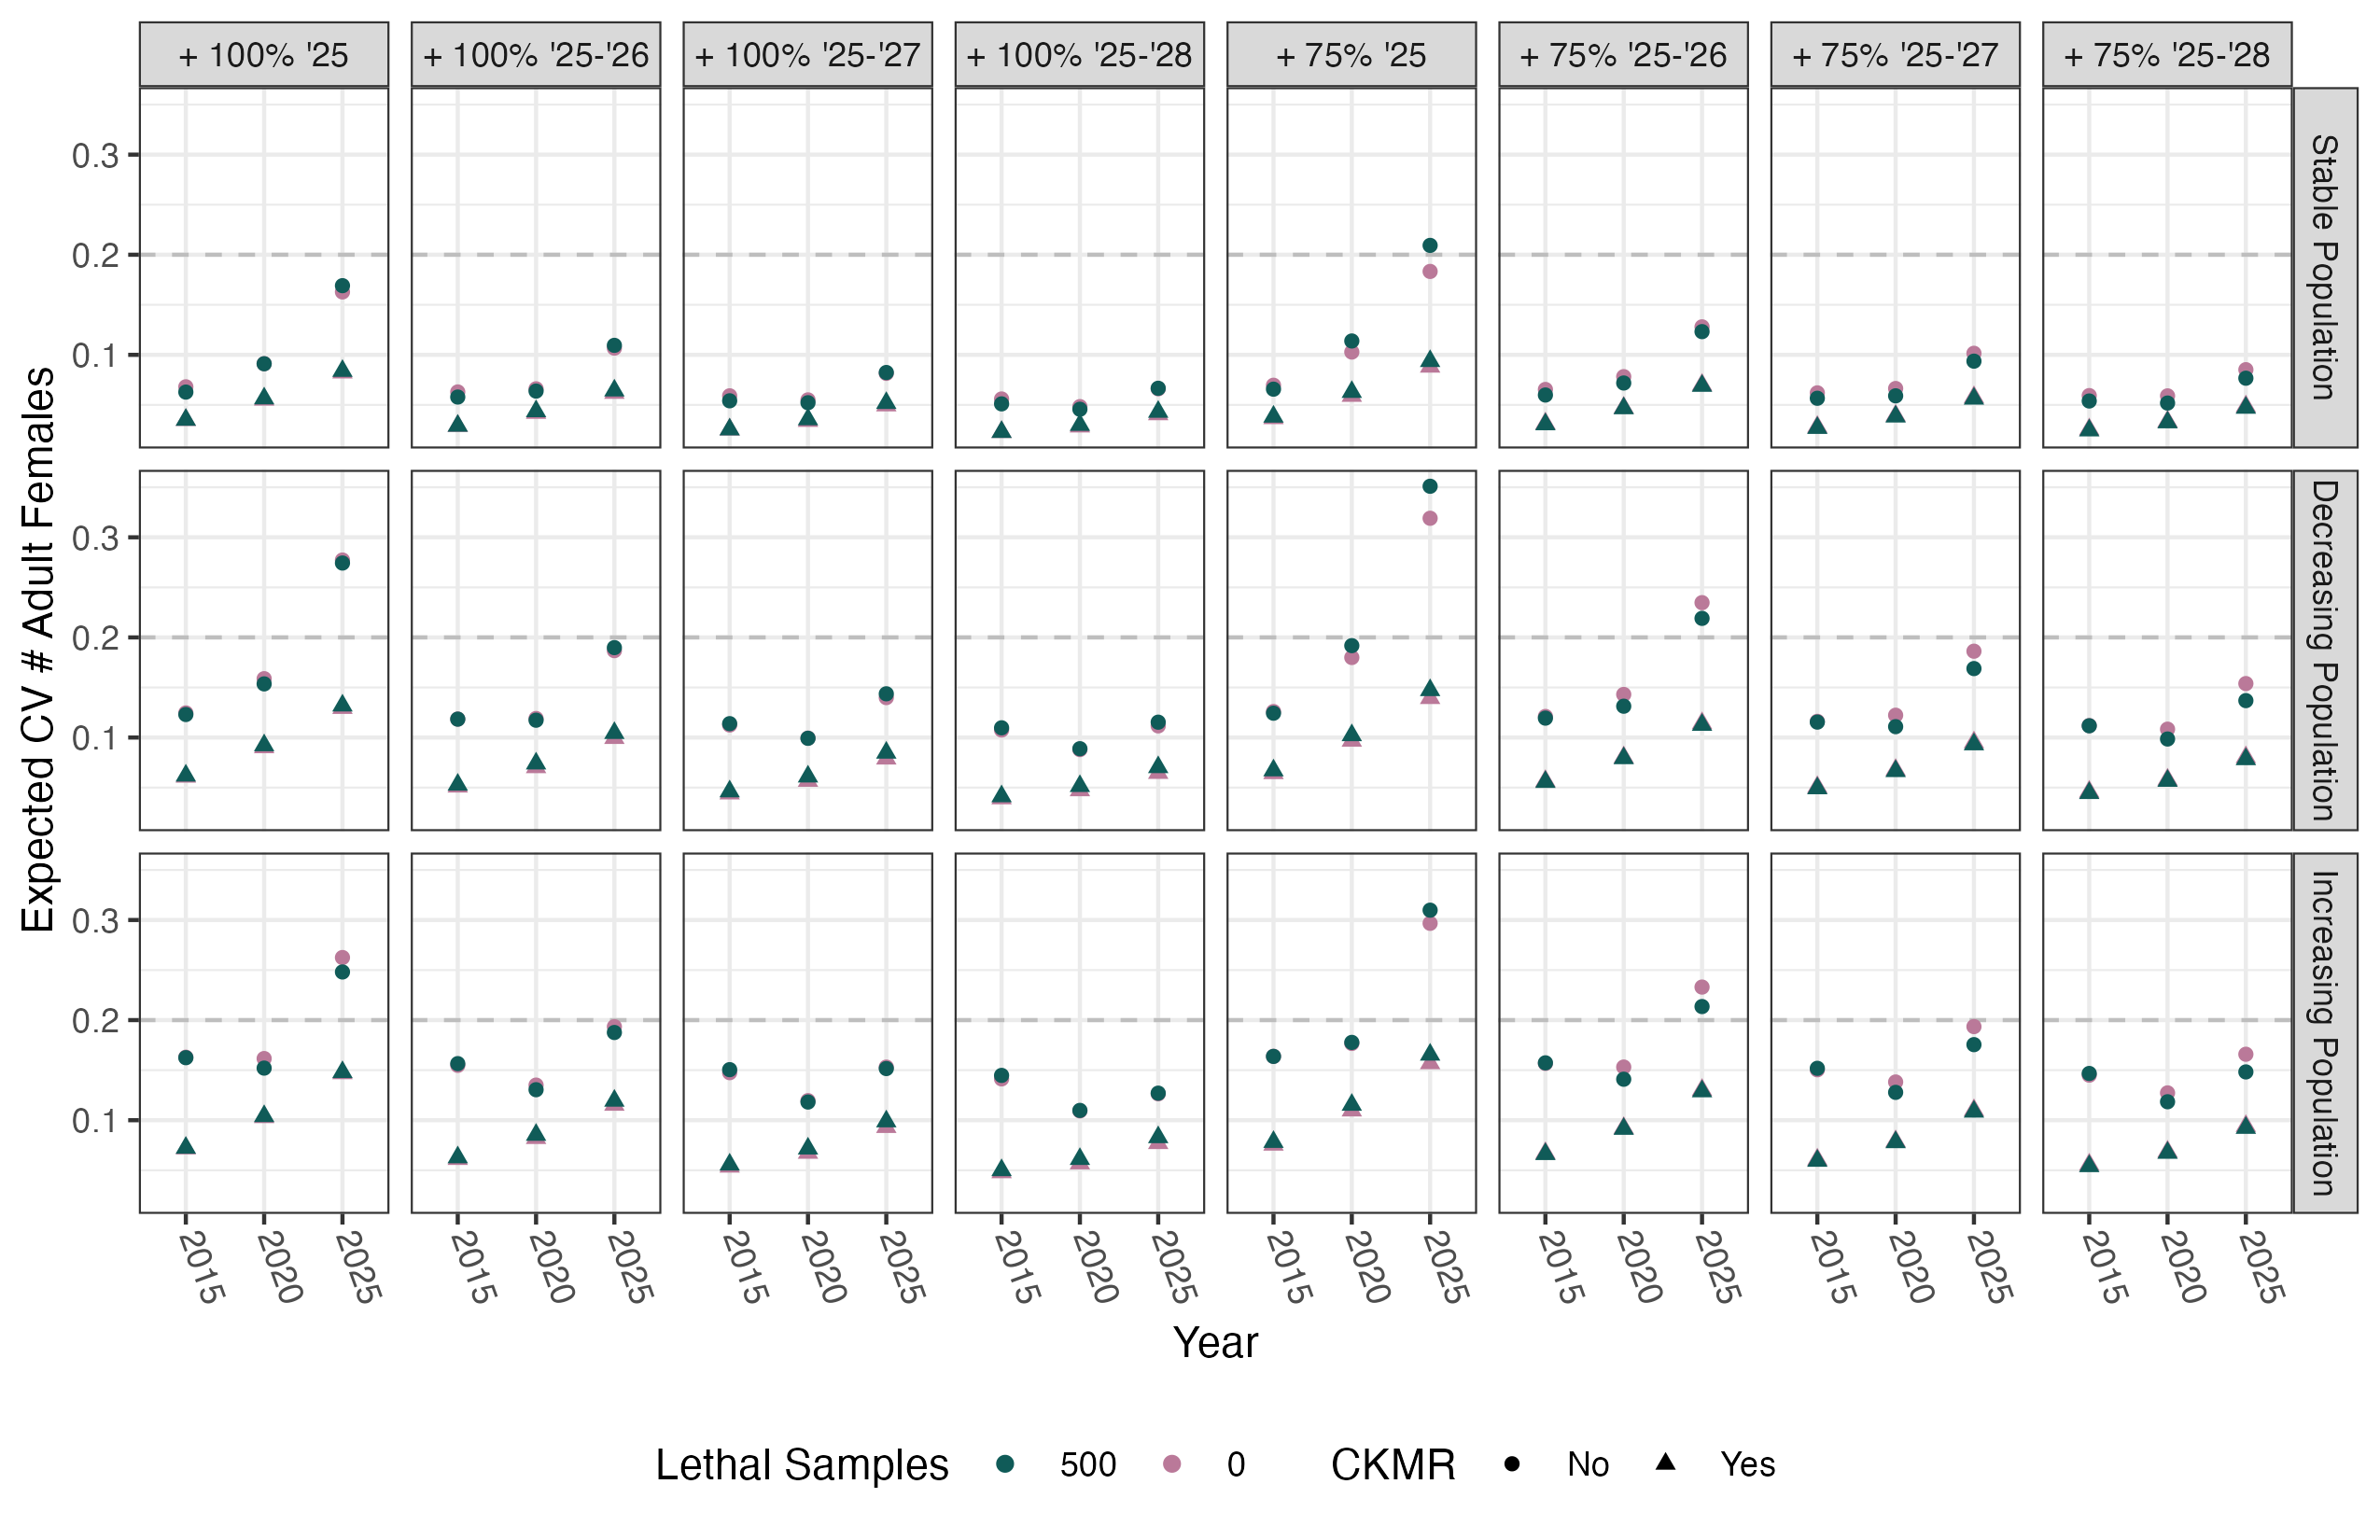
\includegraphics[scale=0.7]{../figures/MegaResults}

\caption{Expected CV of adult female abundance (vertical axis) in different
years (horizontal axis) under different demographic (panel rows) and
sampling (panel column) scenarios. Triangular points represent expected
CVs from IMR alone, while circular points show expected CVs with ICKMR.
The inclusion of lethal samples is indicated by green (lethal samples
included) or purple (no lethal samples included in sampling years)
points. The horizontal dashed line at CV = 0.2 represents an arbitrary
threshold for decision making.\label{fig:megaCV}}
\end{figure}

\begin{figure}
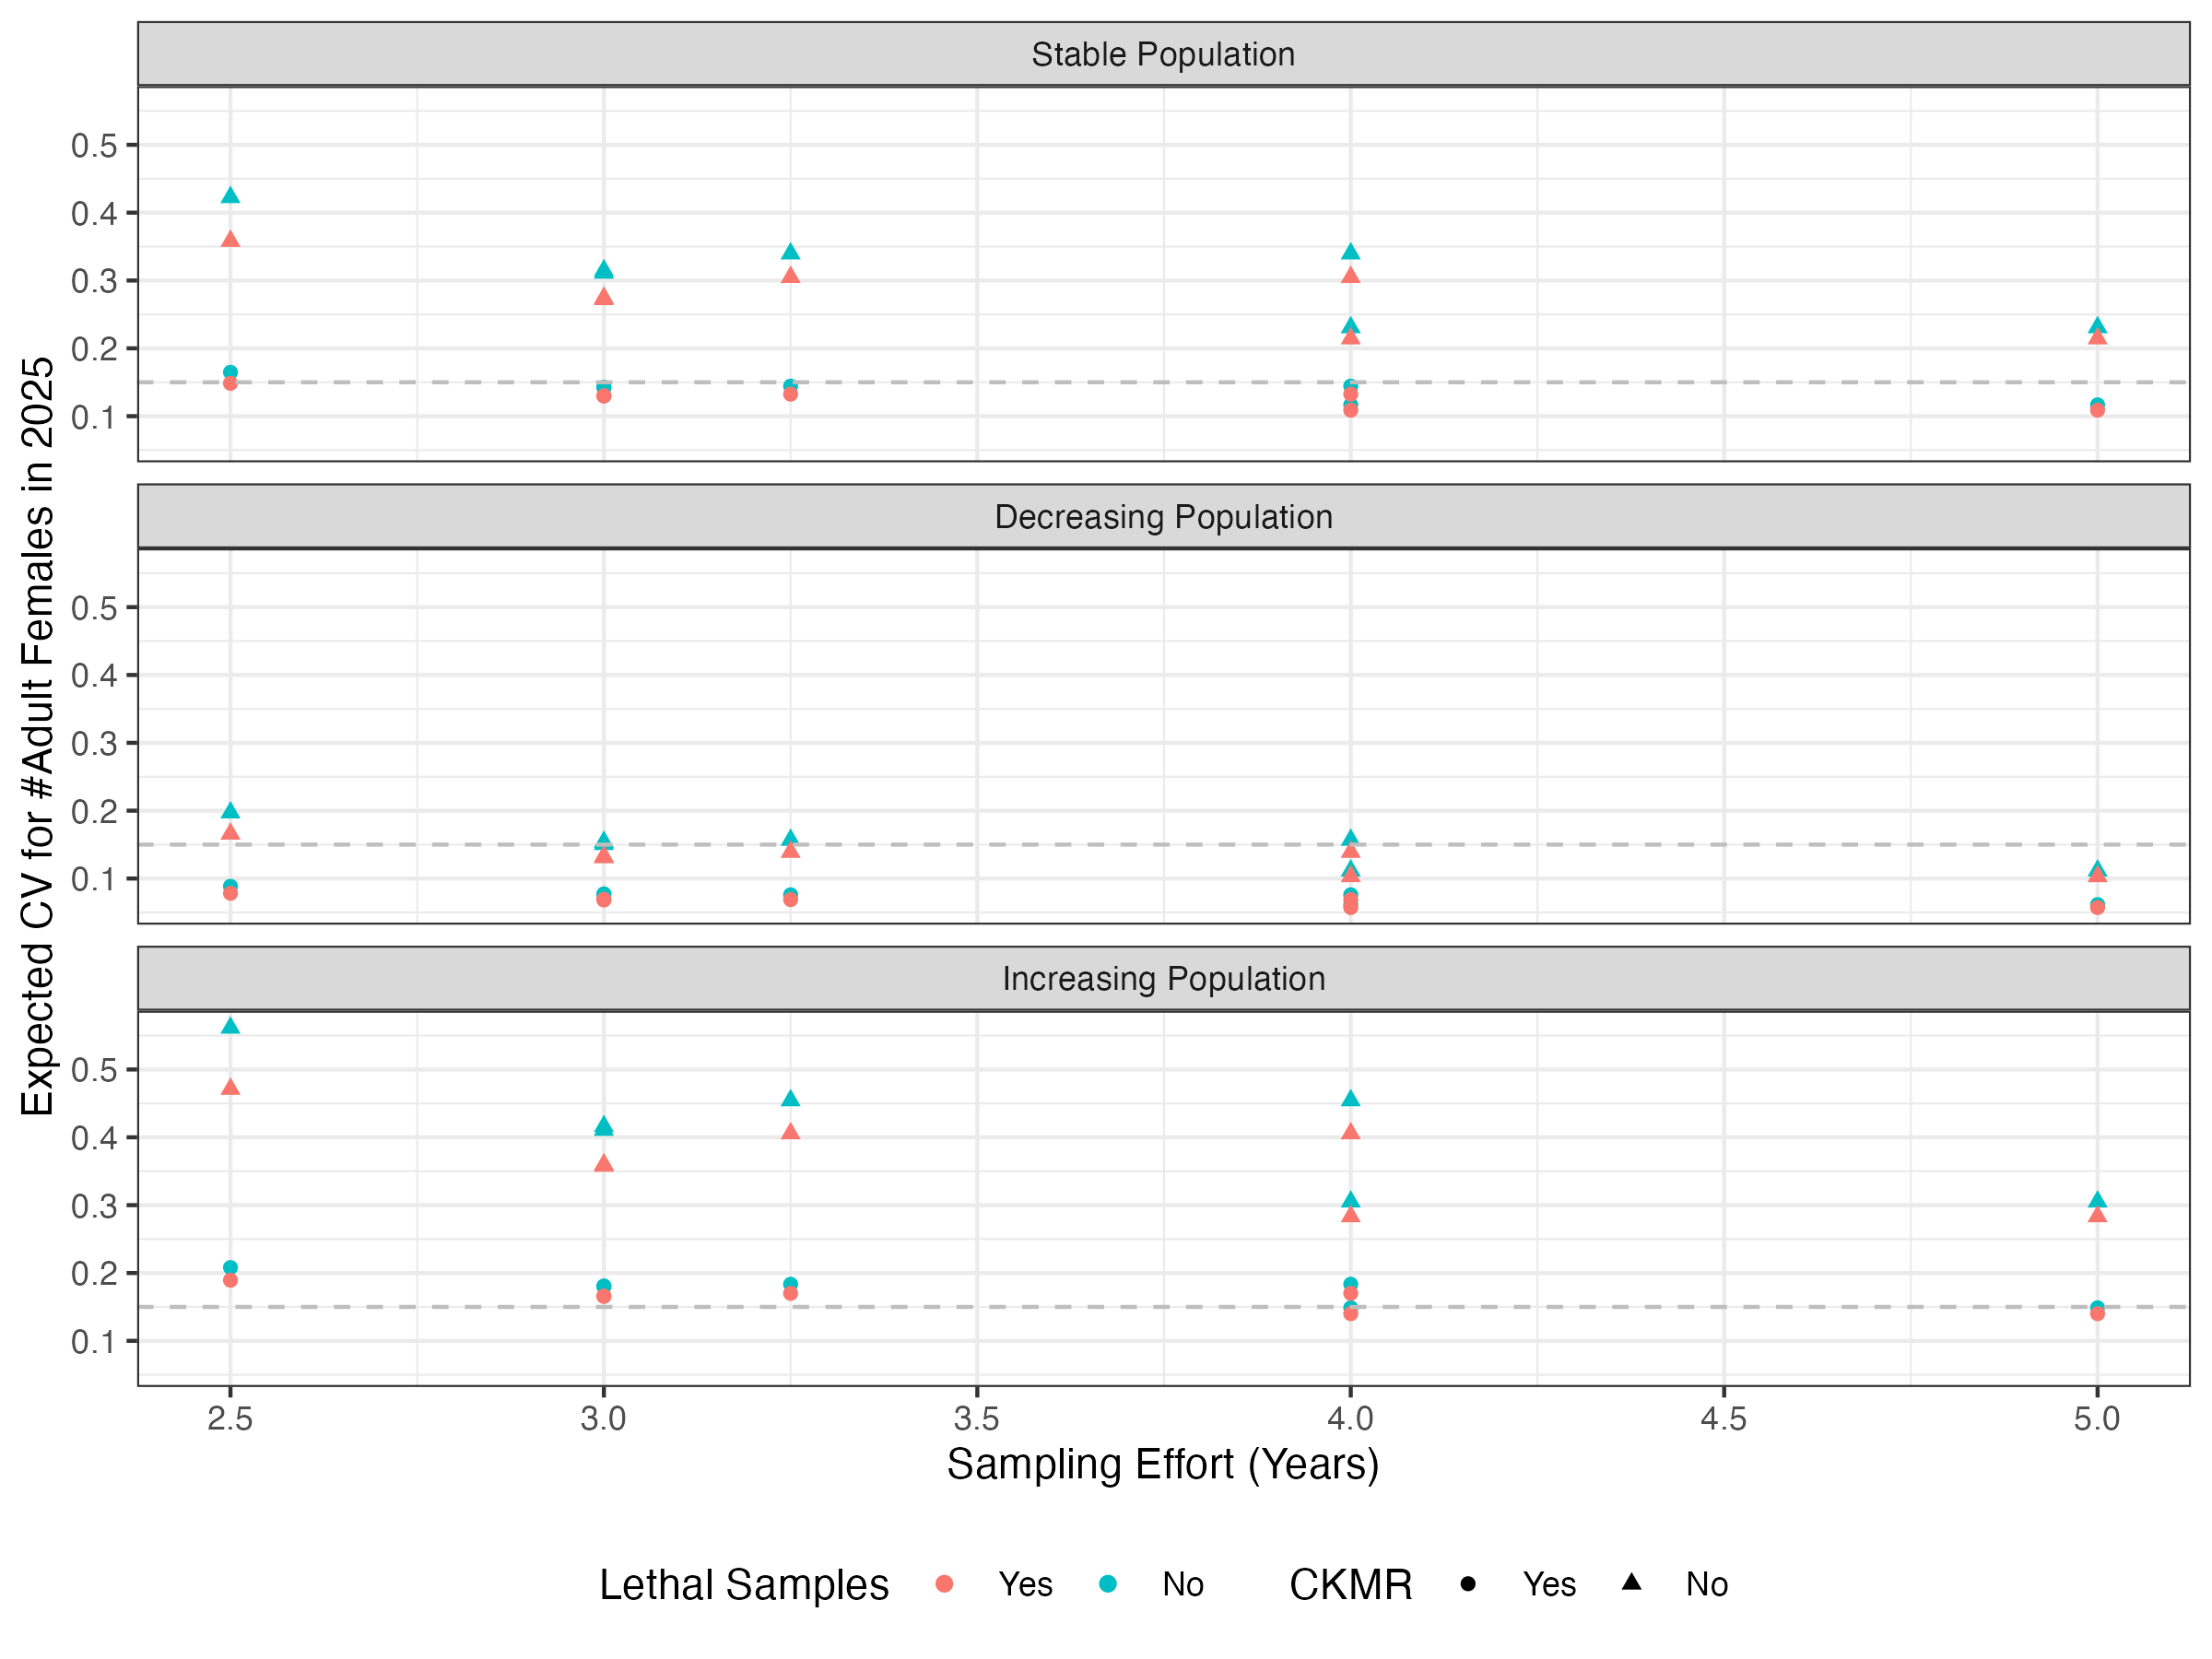
\includegraphics[scale=0.7]{../figures/EffortVCV}

\caption{Sampling effort (in number of years, horizontal axis) versus expected
CV for adult female abundance in 2025 with IMR alone (triangular points)
or with ICKMR (round points) and with (green points) and without (purple
points) the inclusion of lethal samples in sampling years. The three
panels represent demographic scenarios of a stable population, decreasing
population, and increasing population, respectively. The horizontal
dashed line at CV = 0.2 represents an arbitrary threshold for decision
making.\label{fig:effVcv}}
\end{figure}

\begin{figure}
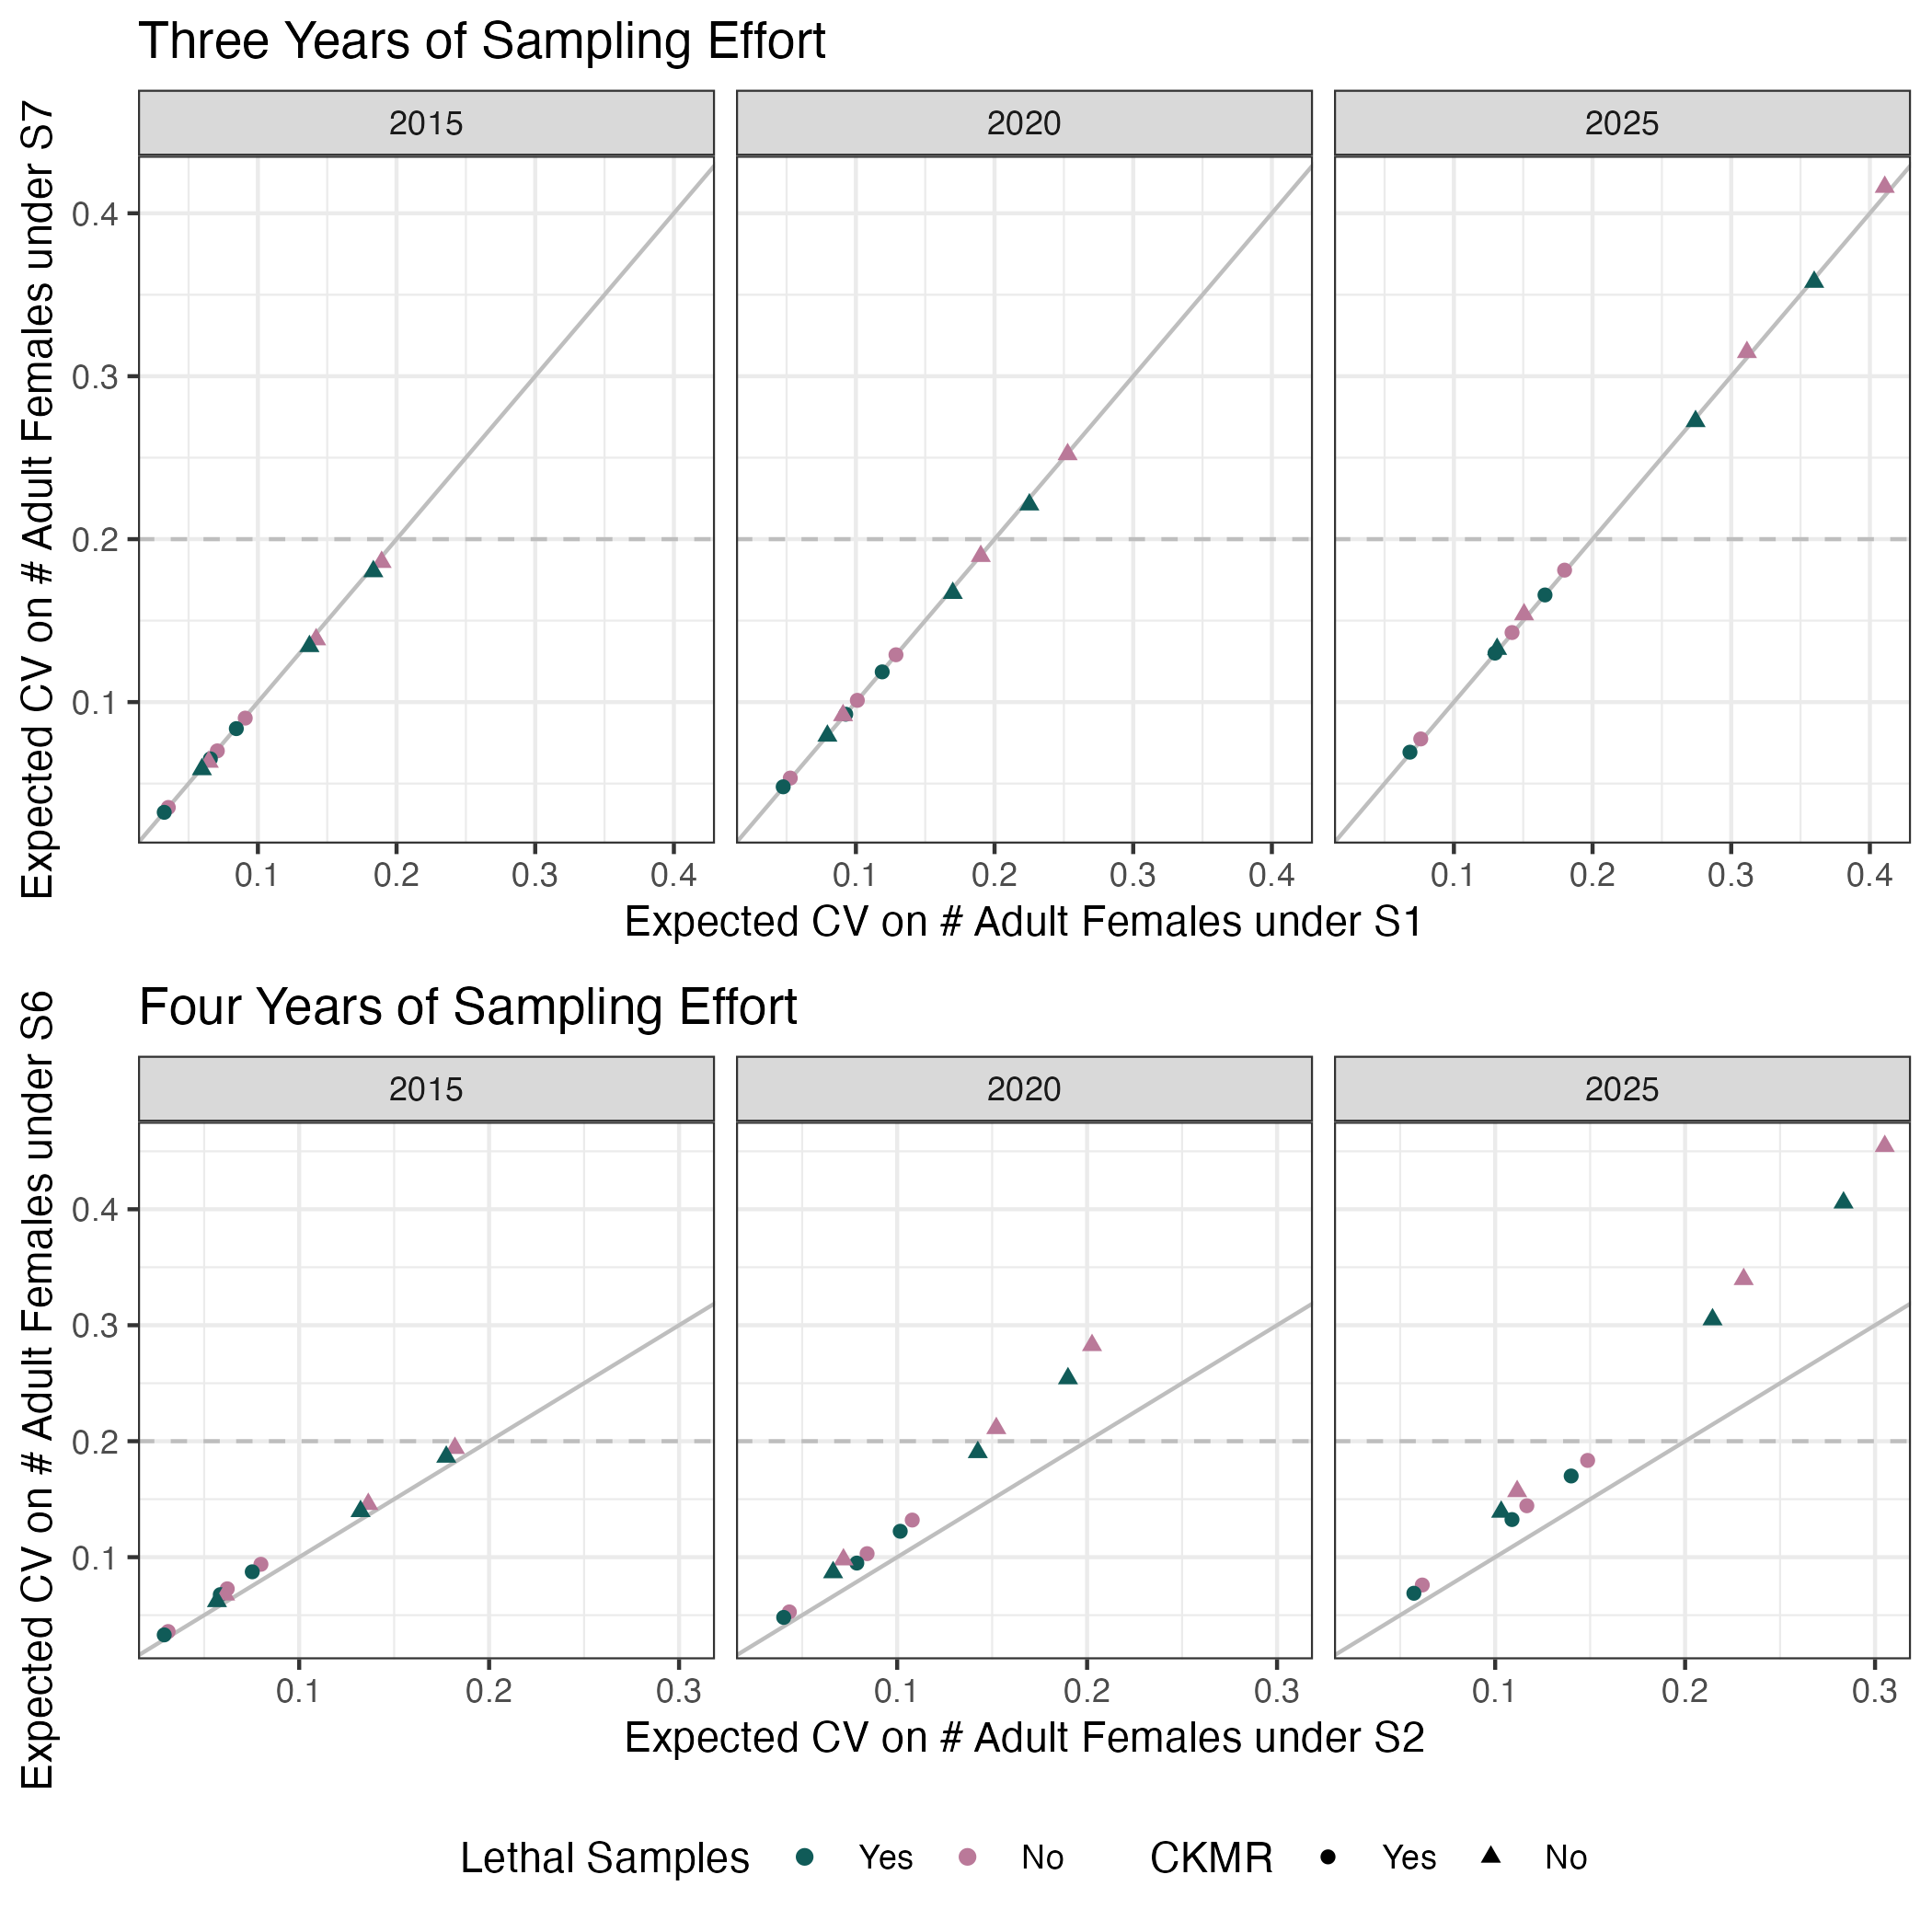
\includegraphics[scale=0.7]{../figures/CVsSameEffort}

\caption{Expected CV on the number of adult females with three years of sampling
(top panels) and four years of sampling (bottom panel). In the top
panel, the horizontal axis shows expected CVs under sampling scenario
1 and the vertical axis shows expected CVs under sampling scenario
7. In the bottom panels, the horizontal axis shows expected CVs under
sampling scenario 2 and the vertical axis shows expected CVs under
sampling scenario 7. From left to right, panels indicate expected
CVs in 2015, 2020, and 2025. Individual points represent expected
CVs under different possible demographic scenarios, with (green) and
without (purple) the inclusion of lethal samples, and with (round
points) and without (triangular points) the use of CKMR (versus IMR
alone). The solid grey line is 1:1. The horizontal dashed grey line
represents an arbitrary threshold CV of 0.2.\label{fig:cvWsameeff}}
\end{figure}

Across all demographic and sampling scenarios, the application of
ICKMR resulted in lower expected precision in estimates of abundance
compared to the application of IMR alone (Fig. \ref{fig:megaCV}).
The mean gain in CV on adult female abundance in paired scenarios
with and without ICKMR was 11\% for a stable population, 5\% for a
decreasing population, and 15\% for an increasing population. See
Table \ref{tab:N_Expected-CV} for expected CVs of adult female abundance
across all demographic and sampling scenarios with and without the
use of ICKMR.

The demographic scenarios (see Table \ref{tab:demo-pars}) affected
expected precision of simulated survey designs in that a decreasing
population resulted in a smaller population size in the years of desired
inference (2015-2025) and therefore the number of kin pairs was higher
(and expected precision was lower) given a set number of samples (Fig.
\ref{fig:megaCV}, second row). Conversely, with an increasing population
size, the number of kin pairs resulting from a set number of samples
was lower, and therefore expected precision was higher (Fig. \ref{fig:megaCV},
third row). With an arbitrary target CV of 0.2 on estimates of adult
female abundance in 2015, 2020, and 2025, all demographic and sampling
scenarios resulted in sufficient precision when the population was
decreasing, while scenarios including ICKMR would be required to achieve
sufficient precision when the population was increasing. 

Lethal samples provided greater gains in precision on abundance estimates
when only IMR was used; the mean gain in precision was 2\% when only
IMR was used but 1\% when ICKMR was applied. Note that when lethal
samples were included, we simulated the collection of 100 lethal samples
per year. We would expect the gain in precision for both IMR and ICKMR
to increase with an increased number of lethal samples. 

The simulated sampling scenarios resulted in between 2.5 and 5 years
of survey effort, where 5 years of survey effort was the original
plan for IMR (Fig. \ref{fig:effVcv}). When the population was simulated
to be stable or decreasing, sufficient precision in abundance estimates
could be achieved with as few as 2.5 years of survey effort when ICKMR
was applied and lethal samples were used. However, in scenarios when
the population was increasing, 4-5 years of survey effort would be
required even with the application of ICKMR and use of lethal samples. 

Some scenarios resulted in the same total number of years of sampling
but in different configurations (i.e., some had more calendar years
with less effort each year whereas others had fewer calendar years
with more effort each year). Scenarios 1 and 7 both resulted in 3
years of survey effort, while sampling scenarios 2 and 6 both resulted
in four years of sampling effort (Fig. \ref{fig:cvWsameeff}). Scenario
1 included sampling effort in 2023, 2025, and 2026, while scenario
7 included sampling in 2023, 2024, and 2025 (see Table \ref{tab:Sampling-scenarios}).
The expected CVs on estimates of adult female abundance in 2025, 2020,
and 2025 were comparable between these sampling scenarios (Fig. \ref{fig:cvWsameeff},
top panel). Scenario 2 included sampling in 2023, 2025, 2026, and
2027, while scenario 6 included sampling in 2023 and a lower level
of sampling (75\% effort) in 2025, 2026, 2027, and 2028. Expected
precision of abundance estimates was greater for scenario 6 than for
scenario 2 in all years of desired inference, with the greatest gains
in the 2025 estimate (Fig. \ref{fig:cvWsameeff}, bottom panel). This
suggests that more years of effort with fewer samples collected per
year could improve overall precision in estimates of adult female
abundance. {[}1204 words{]}.


\section{Discussion}

\selectlanguage{british}%

\begin{itemize}
\item We show how sample collection plans could be modified to achieve desired
monitoring goals with less sampling effort.
\item We didn't bother doing X coz IJAD\footnote{It's Just A Design}. For
real data analysis, we might do Y instead.
\item Ways to extend the model... impact of DNAge
\item Something about adult males and paternal half-siblings (sec 2.1 refers
to discussion)
\item Future utility of lethal samples (although my guess is: there won't
be enough. Glass-half-full, or glass-half-empty, if you're a walrus?)
\item The full ramifications of opting for a stage-structured quasi-equilibrium
model, which avoids having to model age composition but does entail
an \emph{assumption} about selectivity, are not at all obvious, but
the model seems to us fairly reasonable; it might be worth revisiting
when large numbers of DNAge samples become available. At that point
it would be possible to compare the actual age compositions with the
predicted compositions assuming partly-unselective sampling and quasi-equilibrium.
\item on stage-structured dynamics: That assumption may turn out to be unreasonable
for juveniles especially; but it will only be possible to check once
enough sample-age-composition data become available. However, if it
does turn out to be the case that (say) 2yo are disproportionately
likely to be sampled (given their estimated abundance from the fitted
model), then it would not be hard to adjust the stage-structured IMR
equations to incorporate sample-composition-data and (estimated) selectivity.
Sample sizes in this project are large enough that selectivity (i.e.,
the ratio of age-specific sample compositions to model-estimated population
age compositions) should be estimated with respectable precision and
without \textquotedbl propagating\textquotedbl{} a lot of uncertainty
into other parameter estimates. We therefore think that our current
somewhat crude IMR sub-model should give a reasonable guide to ultimate
precision, even if it gets adjusted somewhat in the cold light of
real data. Note that similar assumptions appear to be made in Beatty
et al. 202 (to be confirmed).
\selectlanguage{english}%
\item A purely-age-structured version of \eqref{eq:self-staged} would need
to explicitly keep track of numbers-at-age, not just adult abundance
(as would the other kin types). The quasi-equilibrium assumption might
allow us to do this, but that assumption directly constrains relative
abundances-at-age. In practice, a fully age-structured CKMR formulation
for walrus will need something more sophisticated and time-varying
than a quasi-equilibrium age distribution, and therefore additional
parameters to estimate. We therefore opted for a stage- rather than
age-structured SP model in the hope that the overall statistical information
content about total abundance is reasonably realistic compared to
what we might get from a more complicated population dynamics model.
\item While a stable-age-composition between 2000–2027 is probably not valid
for the entire range of adult ages—since older adults would have experienced
long periods of increased mortality from hunting—it is perhaps a reasonable
assumption for younger adults, and it is only younger adults that
matter here because they indirectly determine the number of juveniles.
A stable age composition for juveniles seems fairly reasonable, since
\textquotedbl recruitment variability\textquotedbl{} cannot be high
for an animal with a litter size of 1, and it only requires a few
years for the juvenile distribution to settle down.
\selectlanguage{british}%
\item As should be evident from the preceding text and number of authors
on this paper, building a close-kin model involves a high level of
collaboration between statisticians, biologists and geneticists. CKMR
is very much a multidisciplinary methodology and each discipline has
a great deal to input into the process of model building.
\item Could mention that CKMR was motivated by fisheries and is an example
of a shared tool between fisheries scientists and ecologists, maybe
cite Schaub et al 2024
\item appendix \eqref{sec:Skip-breeding} discusses skip-breeding\selectlanguage{english}%
\end{itemize}



\printbibliography

\pagebreak{}

\part*{Appendix}

\setcounter{section}{0}
\renewcommand{\thesection}{\Alph{section}}
\numberwithin{equation}{section}

\section{Derivation of self-recapture ``the other way round''}

As discussed in Section \ref{subsec:selfPs}, \eqref{eq:self-staged}
can also be formulated \textquotedbl the other way round\textquotedbl ,
i.e., considering whether the second sample is the same as the first.
The answer turns out the same, but the derivation is slightly different
and \emph{appears} to involve an explicit survival term. Again, suppose
two female samples ($y_{1},a_{1}$ and $y_{2},a_{2}$ , where $y_{1}<y_{2}$),
then 
\begin{gather*}
\mathbb{P}\left[K_{21}=\text{SP}\vert y_{1},a_{1},y_{2},a_{2}\right]\\
=\frac{\mathbb{P}\left[\text{Sample 1 survived until Sample 2 was taken}\right]\mathbb{I}\left(y_{2}-a_{2}=y_{1}-a_{1}\right)}{N\left(y_{2},a_{2}\right)}\\
=\frac{\Phi\left(y_{2}-y_{1},a_{1}\right)\mathbb{I}\left(y_{2}-a_{2}=y_{1}-a_{1}\right)}{N\left(y_{2},a_{2}\right)}.
\end{gather*}

However, the results are readily seen to be identical because, by
definition of \textquotedbl survival\textquotedbl , we have
\begin{gather}
N\left(y+t,a+t\right)\equiv N\left(y,a\right)\Phi\left(t,a\right).\label{eq:cons-of-nums}
\end{gather}

\pagebreak{}

\section{Self-recapture when exact age is known\label{subsec:selfP-exact-age}}

\citet{beatty_estimating_2022} used a fairly complex IMR formulation
to cope with historically-very-imprecise estimates of age (or, more
realistically, of \textquotedbl stage\textquotedbl ) estimates.
However, when accurate age data are available, the pairwise comparison
probabilities for self-recapture are remarkably simple. Suppose two
female samples ($y_{1},a_{1}$ and $y_{2},a_{2}$ , where $y_{1}<y_{2}$).
Then the probability that the first one is the same as the second
is just
\begin{gather}
\mathbb{P}\left[K_{12}=\text{SP}\vert y_{1},a_{1},y_{2},a_{2}\right]=\frac{\mathbb{I}\left(y_{2}-a_{2}=y_{1}-a_{1}\right)}{N_{y_{1},a_{1}}}.\label{eq:SP}
\end{gather}
The indicator $\mathbb{I}\left(\cdot\right)$ is 1 if the two samples
were born in the same year, or 0 if not, The samples can only be from
the same animal if they were both born in the same year and if they
were, we then need to know how many females of age $a_{1}$ were alive
at $y_{1}$, $N_{y_{1},a_{1}}$. This implicitly assumes that all
females of the same age have the same survival and sampling probabilities.
(See appendix for the equivalent derivation of $\mathbb{P}\left[K_{21}=\text{SP}\vert y_{1},a_{1},y_{2},a_{2}\right]$).

In principle, given unlimited data, we could separately apply \eqref{eq:SP}
to each combination of $\left(y,a\right)$-consistent pairs, to empirically
estimate from all numbers-at-age-and-year from the reciprocal of the
observed rates. Then we could apply \eqref{eq:cons-of-nums} to estimate
year-and-age-specific survivals. In practice, that would be ridiculous,
since it would require an enormous number of recaptures and would
lead to noisy abundance estimates, estimated survivals greater than
one, and so on. However, the principle does illustrate the great power
of \emph{known-age} mark-recapture data. Note also that there are
no assumptions about equiprobable sampling across ages, etc; all probabilities
are simply conditioned on observed ages, and it does not particularly
matter \emph{why} there are more samples of one age than another.

The big problem with applying \eqref{eq:SP} in an ICKMR setting,
i.e., with conditioning on age explicitly, is that it requires explicit
calculation of all $N_{y_{1},a_{1}}$ within the model. This is normally
unnecessary with CKMR for mammal-like species, where the main information
is \emph{only} connected with aggregate adult abundance (via TRO).
It is extremely convenient to work just with a \textquotedbl homogenous
block\textquotedbl{} of adults, and there is in any case no direct
information on population age composition unless extra data are used.
One option is \textquotedbl just\textquotedbl{} to work with a fully-age-structured
population dynamics framework— but that is a lot of work to develop
(from experience in fisheries work) and requires modelling extra data.\pagebreak{}

\section{Derivation of juvenile abundance\label{sec:Deriv-Njy}}

The key point here is that we don't need to decompose the adult stage
into separate age classes.

Following notation from the rest of the paper, let the number of adults
in year $y$ be $N_{\text{A},t}$ where adulthood means being aged
$\alpha$ or older. The number next year will be $\rho N_{\text{A},y+1}$
where $\rho=e^{r}$ and $r$ is the rate of increase as in \eqref{popdyn}.
That will be made up of survivors from adults at $t$, plus survivors
from the incoming cohort of oldest juveniles, aged $\alpha-1$. Thus
\begin{gather}
N_{y+1,\text{A}}=\rho N_{y,\text{A}}=\phi_{\text{A}}N_{y,\text{A}}+\phi_{\text{J}}N_{y,\alpha-1}.\label{eq:mvb-nj-1}
\end{gather}
Rearranging, we have
\begin{gather}
N_{y,\alpha-1}=\frac{\rho-\phi_{\text{A}}}{\phi_{\text{J}}}N_{y,\text{A}}.\label{eq:mvb-nj-final-juve}
\end{gather}
We now need to infer the numbers in the other juvenile age-classes
(not just $\alpha-1$). Starting with the penultimate juvenile age-class,
we have: 
\begin{align*}
N_{y,\alpha-1} & =\phi_{\text{J}}N_{y-1,\alpha-2} & \text{ (survival)}\\
N_{y,\alpha-1} & =\rho N_{y-1,\alpha-1} & \text{ (population growth)}\\
\implies N_{y,\alpha-2} & =\frac{\rho}{\phi_{\text{J}}}N_{y,\alpha-1}.
\end{align*}
Similar relationships apply to each preceding juvenile age class,
down to age 1. The total number of juveniles in year $y$, $N_{y,\text{J}}$,
is given by a sum from age $x=\alpha-1$ down to age 1:
\begin{align}
N_{y,\text{J}}=\sum_{x=1}^{\alpha-1}N_{y,\alpha-x} & =\sum_{x=1}^{\alpha-1}N_{y,\alpha-1}\left(\frac{\rho}{\phi_{\text{J}}}\right)^{x-1}\nonumber \\
 & =N_{y,\alpha-1}\sum_{x'=0}^{\alpha-2}\left(\frac{\rho}{\phi_{\text{J}}}\right)^{x'}\nonumber \\
 & =N_{y,\alpha-1}\frac{1-\left(\rho/\phi_{\text{J}}\right)^{\alpha-1}}{1-\rho/\phi_{\text{J}}},\label{eq:mvb-nj-totjuve}
\end{align}
using the standard result for a geometric series: $\sum_{i=1}^{n}ar^{i}=a\frac{1-r^{n}}{1-r}$.
Substituting for $N_{t,\alpha-1}$ from \eqref{eq:mvb-nj-final-juve},
we have
\begin{align*}
N_{y,\text{J}} & =N_{y,\text{A}}\frac{\rho-\phi_{\text{A}}}{\phi_{\text{J}}}\frac{1-\left(\frac{\rho}{\phi_{\text{J}}}\right)^{\alpha-1}}{1-\frac{\rho}{\phi_{\text{J}}}}\\
 & =N_{y,\text{A}}\frac{\rho-\phi_{\text{A}}}{\rho-\phi_{\text{J}}}\left(\left(\frac{\rho}{\phi_{\text{J}}}\right)^{\alpha-1}-1\right).
\end{align*}
Now, for the case of walrus, we know that $\alpha=6$, so:
\begin{align*}
N_{y,\text{J}} & =N_{y,\text{A}}\frac{\rho-\phi_{\text{A}}}{\rho-\phi_{\text{J}}}\left(\left(\frac{\rho}{\phi_{\text{J}}}\right)^{5}-1\right).
\end{align*}
\pagebreak{}

\section{Further HSP complications}

The second issue with all second-order kin, is that pairwise-kinship
statistics are not currently powerful enough to completely distinguish
them all from a few ``lucky'' third-order kin such as Great-Gandparent-Grandchild.
To handle this without bias, the best approach is set a threshold
for the statistic that should almost completely exclude false-positives
from third-order kin, then to estimate empirically the proportion
of true second-order kin that will be lost below the threshold (i.e.,
the false-negative rate) based on the observed distribution of kin-pair
statistics. Only kin-pairs that are above the threshold will be treated
as HSPs, but the probability formula can be multiplied by the complement
of the false-negative probability to compensate. See \citet{bravington_close-kin_2016}
or \citet{Hillary2018WS-CKMR} for more details. The false-negative
rate depends both on the species and the genotyping method (in particular,
the number of loci) and cannot be predicted in advance, but experience
suggests that 15\% is usually a safe upper limit.

Determining that a pair is HSP does not differentiate between mHSPs
(maternal; shared mother) and pHSPs (paternal; shared father). This
can be determined by genotyping the mitochondrial DNA (mtDNA; always
inherited from the mother only) of known HSPs. If the genotypes are
different, the descent must be paternal; if the same, descent is probably
maternal, but could arise by chance in a few paternal-HSP cases. However,
in our experience, except for very small populations (hundreds of
adults), mtDNA diversity has always been high enough that shared-mtDNA
HSPs might as well be treated as definite mHSPs. We assume as much
here.

\pagebreak{}

\section{Adjustments for non-sparse sampling\label{appendix:Adjustments-for-non-sparse}}

Use of the pseudo-log-likelihood Hessian to approximate the inverse
variance is not strictly justified in a mathematical sense, because
the pairwise comparisons are not fully mutually independent. The ``sparse
sampling'' assumption of \citet{bravington_close-kin_2016}, which
underlies the use of the Hessian, is therefore not strictly justified;
this does not lead to bias in point estimates, but the Hessian-based
approximation is likely to underestimate the true variance somewhat.
Accordingly, we have made some simple adjustments to ``effective
sample size'' based on summaries of the simulated datasets. This
should be quite adequate for design purposes— since, in any case,
all our variance estimates have to be based on uncertain assumptions
about true parameter values— but a more detailed treatment may be
worthwhile when it comes to analysing the real data.

A general and comprehensive treatment of non-independence in CKMR
is beyond the scope of this paper. We restrict attention to some obvious
aspects for walrus that are easy to address. We consider the comparisons
in stages: SPs, then MOPs, then XmHSPs. We adjust set the effective
sample size for each stage based on recaptures from the preceding
stages in one simulated dataset, as follows:
\begin{itemize}
\item Sample sizes are initially taken from the simulated dataset (thus
allowing detailed breakdown of sample size by age, year, etc). All
available samples are used for SP comparisons.
\item If an individual is self-recaptured, only its final capture will be
used in MOP and XmHSP comparisons (i.e. duly adjusting the sample
sizes sample sizes for MOPs and XmHSPs, as well as the number of MOPs
etc found if that individual is involved).
\item Any Offspring $o$ identified in a MOP, will be excluded from XmHSP
comparisons (since $o$'s sibship with any other sample $i$ can be
deduced from the MOP results, based on whether $i$ is also an offspring
of $o$'s Mother).
\end{itemize}
This deals with the implications of one type of kinship for the others,
but does not deal with multiple recaptures within a kinship class
(e.g. an individual who is sampled 3 times; given that sample A matches
sample B, and B matches C, it is redundant to compare A with C). There
are simple ways to handle that with real datasets, as long as age
is known fairly accurately.

\pagebreak{}

\section{Model checking\label{sec:Model-checking}}

Close-kin pairwise probability formulae are usually quite simple,
at least with hindsight, but they still can be awkard to get right
in the first place. One way to reduce the risk of mistakes is to generate
simulated datasets, and check that the CKMR code is giving the expected
results when known parameter values are inserted. CKMR simulation
code looks utterly different from kinship-probability code, and the
chance of ``making the same mistake twice'' is therefore much less
than with many statistical simulations. Robustness is improved even
further if two different people are involved, one to simulate and
one to write kinship-probability code. Even though simulation is not
strictly necessary for most CKMR design exercises, simulation may
be worth the additional effort in order to help the whole process,
and that is the approach we took for walrus. We did find and fix several
mistakes this way, both in the CKMR code and in the simulation code,
so the exercise was certainly worthwhile.

The obvious question is how to approach CKMR model-checking when simulated
datasets are available. There are various options and no . One thing
to avoid, if possible, is the naive and laborious approach of actually
\emph{fitting} a CKMR to each simulated dataset, which can be painfully
slow. %
\begin{lyxgreyedout}
(Note, perhaps for discussion: We started this project before RTMB
became available, expecting that the actual model-fitting code for
real data would eventually have to be written in TMB itself, but keen
to avoid the complexity of TMB at the design stage. In contrast, design
calculations are quick because it is only necessary to calculate probability
arrays once, and R alone is adequately fast, without TMB or RTMB.
However, it would not be practical to fit even our simple model to
multiple datasets without RTMB; and even with RTMB, repeated fitting
of a more complicted model, e.g. with copious random effects, might
be a challenge.)%
\end{lyxgreyedout}
{} We used several checks. All are aimed at detecting gross errors (and
we did find some); power to detect subtle mistakes is lower, but in
our experience subtle mistakes are actually less likely than big ones.
The first two checks are based on single realizations of simulated
data, and so are also suitable as diagnostics when fitting to real
data; the last two require multiple simulated datasets.

\begin{comment}
One option is to include final result(s) for each check right here,
after describing the check. Otherwise, if this section goes mainly
into Methods, the results of each little check will be a long way
from the text describing it, and the reader will have forgotten what
the check is by the time they see its results. I absolutely hate papers
like that :) But, it might depend; needs Zoom.
\end{comment}

\begin{itemize}
\item Observed and expected totals of sampled kin-pairs of each type. Clearly,
unless these match reasonably well, there must be a major inconsistency
between model and simulationg. The definition of ``reasonably well''
can be guided by the inherent Poisson variability. If an expected
total is 227, say, then we would not expect to see observed total
much outside, say, the 95\% confidence limits for a Poisson distribution
with mean (and therefore variance) 227. This can be roughly approximated
by $227\pm2\sqrt{227}$ or about {[}195,255{]}. Clearly, the expected
total needs to be fairly large for this to have much power, so it
might be useful to increase the simulated sample size for checking
purposes.\\
{*}{*}OPTION{*}{*}list the totals here (for first test dataset, chosen
so that sim matches CK code as closely as possible)
\item Breakdown of observed and expected kin-pair totals across some covariate
of interest. If the totals from the previous step are not matching
well, then the breakdown may shed light on where to look for problems.
For example: the distribution of birth-gaps between XmHSPs is driven
in the longer term by the adult rate mortality rate, so if observed
and expected do not correspond, then the treatment of mortality is
likely inconsistent. Also, the number of mothers by age-at-birth should
fluctuate over the first few years of adulthood because of the typically-three-year
breeding cycle (most 6yo have just given birth; most 7yo are still
nursing last year's offspring, etc), until it settles down because
of the averaging effects of irregularities. If the observed and expected
patterns do not match, then the breeding cycle treatment is inconsistent.\\
{*}{*}OPTION{*}{*} show the 2 graphs here.
\item P-values of observed kin-totals by type, based on the Poisson distribution
as above. Given a reasonable number of simulated datasets (say 20
or more), these should be roughly uniform across the interval {[}0,1{]}.
Clearly, it would require a large number of simulations to get a precise
check here, but precision is not necessary: the goal is to pick up
fairly coarse errors.\\
{*}{*}OPTION{*}{*} show 4 histos here (instead of box'n'whiska)
\item Looking at the mean and variance of the derivative of the pseudo-log-likelihood
at the true parameter values $\theta_{0}$ (something which can be
calculated fairly quickly by numerical differentiation). The mean
should be close to 0 and the variance determines what ``close''
might mean, given the number of simulations available. This checks
the crucial ``unbiased estimating equation'' (UEE) assumption required
by most statistical estimation frameworks, including maximum-likelihood.
If UEE does not hold, then by definition there is a mismatch between
simulation and model.\\
{*}{*}OPTION{*}{*} there's some numbers printeed at the end of compare2sims.R,
I thnk.
\end{itemize}
The description so far implicitly assumes that the CKMR model (if
working right) corresponds exactly to the data-generation mechanism
in the simulations. However, it might be desirable to make the CKMR
model simpler, especially for design purposes where the goal is just
to make sure that sampling plans are sensible; developing a more complicated
and realistic model can often be left until the real data appears.
For example, we wanted to avoid reproductive senescence in the CKMR
equations, so that all adults could be treated as a single block without
requiring age-structured dynamics inside the model. Nevertheless,
senescence is likely a reality of the walrus world, and there is such
a thing as ``too simple to be useful'', so it is worth checking
whether the simpler formulation is going to run into serious trouble.
Simulated datasets can be used to estimate approximate bias in a slightly-mis-specified
CKMR model, again without needing to do any estimation. The idea is
to approximate the MLE for each dataset, based only on calculations
using the true parameter value for the simulations. The MLE $\hat{\theta}$
will by definition satisfy the equation $\left.d\Lambda/d\theta\right\vert _{\hat{\theta}}=0$,
and we can take a first-order Taylor expansion around the true value
$\theta_{0}$ to give

\begin{gather}
0=\left.\frac{d\Lambda}{d\theta}\right\vert _{\hat{\theta}}\approx\left.\frac{d\Lambda}{d\theta}\right\vert _{\theta_{0}}+\left(\hat{\theta}-\theta_{0}\right)\left.\frac{d^{2}\Lambda}{d\theta^{2}}\right\vert _{\theta_{0}}\nonumber \\
\implies\hat{\theta}-\theta_{0}\approx-\left[\left.\frac{d\Lambda^{2}}{d\theta^{2}}\right\vert _{\theta_{0}}\right]^{-1}\left.\frac{d\Lambda}{d\theta}\right\vert _{\theta_{0}}\label{eq:bias-approx}
\end{gather}

The square-bracketed term can be replaced (to the same order of accuracy
as the rest of the approxmation) by the \emph{expected} Hessian which
is the crux of our design calculations anyway, and which of course
does not vary from one simulation to the next. Thus, the only quantity
that has to be calculated per simulated dataset is $\left.d\Lambda/d\theta\right\vert _{\theta_{0}}$,
already required for the unbiased-estimating-equation check above.
The estimated bias is the average across simulations of (\ref{eq:bias-approx}).
This is quite similar to the UEE check above, but with a change in
focus: this time, we may be prepared to tolerate some small violation
of UEE, provided that it does not imply substantial bias on the parameter
scale. In particular, if the estimated bias for the $r$\textsuperscript{th}
parameter (i.e. $r$\textsuperscript{th } component of $\theta$)
is below its sampling variability— say, if bias is less than 1 standard
deviation, computed from the square-root of the diagonal of the inverse
Hessian or $\sqrt{H^{-1}\left(r,r\right)}$— then there is little
reason to worry about bias for that particular parameter. 

{*}{*}OPTION{*}{*} stuff from the end of compare2sims.R

{*}{*}DISCUSSION?{*}{*}

In the end, based on the checks above, our estimation and simulation
codes did indeed appear consistent, and any bias induced by (among
other minor things) ignoring senescence did not seem problematic.
Of course, we only reached that position \emph{after} going thru the
checking process several times, to find and fix inconsistencies.


\pagebreak{}

\section{Additional results\label{sec:Additional-results}}

\selectlanguage{american}%
\begin{table}
\caption{Expected CVs on adult female survival, juvenile female survival, and
the proportion of adult females in breeding state 2 under different
demographic and sampling scenarios with and without the use of lethal
samples and CKMR.\label{tab:LH_Expected-CVs}}

\begin{tabular}{|c|c|c|c|c|c|c|}
\hline 
\begin{cellvarwidth}[t]
\centering
Demographic 

Scenario
\end{cellvarwidth} & \begin{cellvarwidth}[t]
\centering
Lethal 

Samples
\end{cellvarwidth} & \begin{cellvarwidth}[t]
\centering
Sampling 

Scenario
\end{cellvarwidth} & CKMR & \begin{cellvarwidth}[t]
\centering
Adult Female 

Survival
\end{cellvarwidth} & \begin{cellvarwidth}[t]
\centering
Juvenile Female 

Survival
\end{cellvarwidth} & \begin{cellvarwidth}[t]
\centering
P. Adult Female 

in State 2
\end{cellvarwidth}\tabularnewline
\hline 
\hline 
1 & No & 1 & Yes & 0.01 & 0.05 & 0.1\tabularnewline
\hline 
1 & No & 2 & Yes & 0.01 & 0.04 & 0.09\tabularnewline
\hline 
1 & No & 3 & Yes & 0.01 & 0.04 & 0.09\tabularnewline
\hline 
1 & No & 4 & Yes & 0.02 & 0.05 & 0.11\tabularnewline
\hline 
1 & No & 5 & Yes & 0.01 & 0.05 & 0.1\tabularnewline
\hline 
1 & No & 6 & Yes & 0.01 & 0.05 & 0.1\tabularnewline
\hline 
1 & No & 7 & Yes & 0.01 & 0.05 & 0.1\tabularnewline
\hline 
1 & Yes & 1 & Yes & 0.01 & 0.04 & 0.1\tabularnewline
\hline 
1 & Yes & 2 & Yes & 0.01 & 0.04 & 0.09\tabularnewline
\hline 
1 & Yes & 3 & Yes & 0.01 & 0.04 & 0.09\tabularnewline
\hline 
1 & Yes & 4 & Yes & 0.01 & 0.05 & 0.1\tabularnewline
\hline 
1 & Yes & 5 & Yes & 0.01 & 0.04 & 0.1\tabularnewline
\hline 
1 & Yes & 6 & Yes & 0.01 & 0.04 & 0.1\tabularnewline
\hline 
1 & Yes & 7 & Yes & 0.01 & 0.05 & 0.09\tabularnewline
\hline 
2 & No & 1 & Yes & 0.01 & 0.03 & 0.06\tabularnewline
\hline 
2 & No & 2 & Yes & 0.01 & 0.02 & 0.05\tabularnewline
\hline 
2 & No & 3 & Yes & 0.01 & 0.02 & 0.05\tabularnewline
\hline 
2 & No & 4 & Yes & 0.01 & 0.03 & 0.07\tabularnewline
\hline 
2 & No & 5 & Yes & 0.01 & 0.03 & 0.06\tabularnewline
\hline 
2 & No & 6 & Yes & 0.01 & 0.03 & 0.06\tabularnewline
\hline 
2 & No & 7 & Yes & 0.01 & 0.03 & 0.06\tabularnewline
\hline 
2 & Yes & 1 & Yes & 0.01 & 0.03 & 0.06\tabularnewline
\hline 
2 & Yes & 2 & Yes & 0.01 & 0.02 & 0.05\tabularnewline
\hline 
2 & Yes & 3 & Yes & 0.01 & 0.02 & 0.05\tabularnewline
\hline 
2 & Yes & 4 & Yes & 0.01 & 0.03 & 0.06\tabularnewline
\hline 
2 & Yes & 5 & Yes & 0.01 & 0.03 & 0.06\tabularnewline
\hline 
2 & Yes & 6 & Yes & 0.01 & 0.03 & 0.06\tabularnewline
\hline 
2 & Yes & 7 & Yes & 0.01 & 0.03 & 0.06\tabularnewline
\hline 
3 & No & 1 & Yes & 0.02 & 0.06 & 0.13\tabularnewline
\hline 
3 & No & 2 & Yes & 0.02 & 0.05 & 0.11\tabularnewline
\hline 
3 & No & 3 & Yes & 0.02 & 0.05 & 0.11\tabularnewline
\hline 
3 & No & 4 & Yes & 0.02 & 0.07 & 0.14\tabularnewline
\hline 
3 & No & 5 & Yes & 0.02 & 0.06 & 0.13\tabularnewline
\hline 
3 & No & 6 & Yes & 0.02 & 0.06 & 0.13\tabularnewline
\hline 
3 & No & 7 & Yes & 0.02 & 0.06 & 0.12\tabularnewline
\hline 
3 & Yes & 1 & Yes & 0.02 & 0.06 & 0.12\tabularnewline
\hline 
3 & Yes & 2 & Yes & 0.01 & 0.05 & 0.11\tabularnewline
\hline 
3 & Yes & 3 & Yes & 0.01 & 0.05 & 0.11\tabularnewline
\hline 
3 & Yes & 4 & Yes & 0.02 & 0.06 & 0.13\tabularnewline
\hline 
3 & Yes & 5 & Yes & 0.02 & 0.06 & 0.12\tabularnewline
\hline 
3 & Yes & 6 & Yes & 0.02 & 0.06 & 0.12\tabularnewline
\hline 
3 & Yes & 7 & Yes & 0.02 & 0.06 & 0.12\tabularnewline
\hline 
1 & No & 1 & No & 0.03 & 0.07 & 1.01\tabularnewline
\hline 
1 & No & 2 & No & 0.03 & 0.06 & 0.92\tabularnewline
\hline 
1 & No & 3 & No & 0.03 & 0.06 & 0.92\tabularnewline
\hline 
1 & No & 4 & No & 0.04 & 0.08 & 1.1\tabularnewline
\hline 
1 & No & 5 & No & 0.04 & 0.08 & 1.04\tabularnewline
\hline 
1 & No & 6 & No & 0.04 & 0.08 & 1.04\tabularnewline
\hline 
1 & No & 7 & No & 0.03 & 0.07 & 1\tabularnewline
\hline 
1 & Yes & 1 & No & 0.03 & 0.06 & 0.94\tabularnewline
\hline 
1 & Yes & 2 & No & 0.02 & 0.06 & 0.86\tabularnewline
\hline 
1 & Yes & 3 & No & 0.02 & 0.06 & 0.86\tabularnewline
\hline 
1 & Yes & 4 & No & 0.04 & 0.07 & 1.03\tabularnewline
\hline 
1 & Yes & 5 & No & 0.03 & 0.07 & 0.97\tabularnewline
\hline 
1 & Yes & 6 & No & 0.03 & 0.07 & 0.97\tabularnewline
\hline 
1 & Yes & 7 & No & 0.03 & 0.06 & 0.94\tabularnewline
\hline 
2 & No & 1 & No & 0.02 & 0.04 & 0.6\tabularnewline
\hline 
2 & No & 2 & No & 0.01 & 0.03 & 0.54\tabularnewline
\hline 
2 & No & 3 & No & 0.01 & 0.03 & 0.54\tabularnewline
\hline 
2 & No & 4 & No & 0.02 & 0.05 & 0.65\tabularnewline
\hline 
2 & No & 5 & No & 0.02 & 0.04 & 0.61\tabularnewline
\hline 
2 & No & 6 & No & 0.02 & 0.04 & 0.61\tabularnewline
\hline 
2 & No & 7 & No & 0.02 & 0.04 & 0.59\tabularnewline
\hline 
2 & Yes & 1 & No & 0.01 & 0.04 & 0.55\tabularnewline
\hline 
2 & Yes & 2 & No & 0.01 & 0.03 & 0.51\tabularnewline
\hline 
2 & Yes & 3 & No & 0.01 & 0.03 & 0.51\tabularnewline
\hline 
2 & Yes & 4 & No & 0.02 & 0.04 & 0.6\tabularnewline
\hline 
2 & Yes & 5 & No & 0.01 & 0.04 & 0.56\tabularnewline
\hline 
2 & Yes & 6 & No & 0.01 & 0.04 & 0.56\tabularnewline
\hline 
2 & Yes & 7 & No & 0.01 & 0.04 & 0.55\tabularnewline
\hline 
3 & No & 1 & No & 0.04 & 0.09 & 1.25\tabularnewline
\hline 
3 & No & 2 & No & 0.03 & 0.08 & 1.13\tabularnewline
\hline 
3 & No & 3 & No & 0.03 & 0.08 & 1.13\tabularnewline
\hline 
3 & No & 4 & No & 0.06 & 0.11 & 1.36\tabularnewline
\hline 
3 & No & 5 & No & 0.05 & 0.1 & 1.29\tabularnewline
\hline 
3 & No & 6 & No & 0.05 & 0.1 & 1.29\tabularnewline
\hline 
3 & No & 7 & No & 0.04 & 0.09 & 1.24\tabularnewline
\hline 
3 & Yes & 1 & No & 0.04 & 0.08 & 1.17\tabularnewline
\hline 
3 & Yes & 2 & No & 0.03 & 0.07 & 1.07\tabularnewline
\hline 
3 & Yes & 3 & No & 0.03 & 0.07 & 1.07\tabularnewline
\hline 
3 & Yes & 4 & No & 0.05 & 0.09 & 1.27\tabularnewline
\hline 
3 & Yes & 5 & No & 0.04 & 0.09 & 1.21\tabularnewline
\hline 
3 & Yes & 6 & No & 0.04 & 0.09 & 1.21\tabularnewline
\hline 
3 & Yes & 7 & No & 0.04 & 0.08 & 1.16\tabularnewline
\hline 
\end{tabular}
\end{table}

\begin{table}
\selectlanguage{english}%
\caption{Expected CV on adult female population size in 2015, 2020, and 2025
with different demographic and sampling scenarios and with and without
the use of lethal samples and CKMR. \label{tab:N_Expected-CV}}

\begin{tabular}{|c|c|c|c|c|c|c|}
\hline 
\begin{cellvarwidth}[t]
\centering
Demographic 

Scenario
\end{cellvarwidth} & \begin{cellvarwidth}[t]
\centering
Lethal 

Samples
\end{cellvarwidth} & \begin{cellvarwidth}[t]
\centering
Sampling 

Scenario
\end{cellvarwidth} & CKMR & \begin{cellvarwidth}[t]
\centering
2015 

Adult Females
\end{cellvarwidth} & \begin{cellvarwidth}[t]
\centering
2020 

Adult Females
\end{cellvarwidth} & \begin{cellvarwidth}[t]
\centering
2025 

Adult Females
\end{cellvarwidth}\tabularnewline
\hline 
\hline 
1 & No & 1 & Yes & 0.07 & 0.1 & 0.14\tabularnewline
\hline 
1 & No & 2 & Yes & 0.06 & 0.08 & 0.12\tabularnewline
\hline 
1 & No & 3 & Yes & 0.06 & 0.08 & 0.12\tabularnewline
\hline 
1 & No & 4 & Yes & 0.08 & 0.12 & 0.16\tabularnewline
\hline 
1 & No & 5 & Yes & 0.07 & 0.1 & 0.14\tabularnewline
\hline 
1 & No & 6 & Yes & 0.07 & 0.1 & 0.14\tabularnewline
\hline 
1 & No & 7 & Yes & 0.07 & 0.1 & 0.14\tabularnewline
\hline 
1 & Yes & 1 & Yes & 0.07 & 0.09 & 0.13\tabularnewline
\hline 
1 & Yes & 2 & Yes & 0.06 & 0.08 & 0.11\tabularnewline
\hline 
1 & Yes & 3 & Yes & 0.06 & 0.08 & 0.11\tabularnewline
\hline 
1 & Yes & 4 & Yes & 0.07 & 0.11 & 0.15\tabularnewline
\hline 
1 & Yes & 5 & Yes & 0.07 & 0.09 & 0.13\tabularnewline
\hline 
1 & Yes & 6 & Yes & 0.07 & 0.09 & 0.13\tabularnewline
\hline 
1 & Yes & 7 & Yes & 0.07 & 0.09 & 0.13\tabularnewline
\hline 
2 & No & 1 & Yes & 0.04 & 0.05 & 0.08\tabularnewline
\hline 
2 & No & 2 & Yes & 0.03 & 0.04 & 0.06\tabularnewline
\hline 
2 & No & 3 & Yes & 0.03 & 0.04 & 0.06\tabularnewline
\hline 
2 & No & 4 & Yes & 0.04 & 0.06 & 0.09\tabularnewline
\hline 
2 & No & 5 & Yes & 0.04 & 0.05 & 0.08\tabularnewline
\hline 
2 & No & 6 & Yes & 0.04 & 0.05 & 0.08\tabularnewline
\hline 
2 & No & 7 & Yes & 0.04 & 0.05 & 0.08\tabularnewline
\hline 
2 & Yes & 1 & Yes & 0.03 & 0.05 & 0.07\tabularnewline
\hline 
2 & Yes & 2 & Yes & 0.03 & 0.04 & 0.06\tabularnewline
\hline 
2 & Yes & 3 & Yes & 0.03 & 0.04 & 0.06\tabularnewline
\hline 
2 & Yes & 4 & Yes & 0.04 & 0.05 & 0.08\tabularnewline
\hline 
2 & Yes & 5 & Yes & 0.03 & 0.05 & 0.07\tabularnewline
\hline 
2 & Yes & 6 & Yes & 0.03 & 0.05 & 0.07\tabularnewline
\hline 
2 & Yes & 7 & Yes & 0.03 & 0.05 & 0.07\tabularnewline
\hline 
3 & No & 1 & Yes & 0.09 & 0.13 & 0.18\tabularnewline
\hline 
3 & No & 2 & Yes & 0.08 & 0.11 & 0.15\tabularnewline
\hline 
3 & No & 3 & Yes & 0.08 & 0.11 & 0.15\tabularnewline
\hline 
3 & No & 4 & Yes & 0.1 & 0.15 & 0.21\tabularnewline
\hline 
3 & No & 5 & Yes & 0.09 & 0.13 & 0.18\tabularnewline
\hline 
3 & No & 6 & Yes & 0.09 & 0.13 & 0.18\tabularnewline
\hline 
3 & No & 7 & Yes & 0.09 & 0.13 & 0.18\tabularnewline
\hline 
3 & Yes & 1 & Yes & 0.08 & 0.12 & 0.17\tabularnewline
\hline 
3 & Yes & 2 & Yes & 0.08 & 0.1 & 0.14\tabularnewline
\hline 
3 & Yes & 3 & Yes & 0.08 & 0.1 & 0.14\tabularnewline
\hline 
3 & Yes & 4 & Yes & 0.09 & 0.14 & 0.19\tabularnewline
\hline 
3 & Yes & 5 & Yes & 0.09 & 0.12 & 0.17\tabularnewline
\hline 
3 & Yes & 6 & Yes & 0.09 & 0.12 & 0.17\tabularnewline
\hline 
3 & Yes & 7 & Yes & 0.08 & 0.12 & 0.17\tabularnewline
\hline 
1 & No & 1 & No & 0.14 & 0.19 & 0.31\tabularnewline
\hline 
1 & No & 2 & No & 0.14 & 0.15 & 0.23\tabularnewline
\hline 
1 & No & 3 & No & 0.14 & 0.15 & 0.23\tabularnewline
\hline 
1 & No & 4 & No & 0.15 & 0.25 & 0.42\tabularnewline
\hline 
1 & No & 5 & No & 0.15 & 0.21 & 0.34\tabularnewline
\hline 
1 & No & 6 & No & 0.15 & 0.21 & 0.34\tabularnewline
\hline 
1 & No & 7 & No & 0.14 & 0.19 & 0.31\tabularnewline
\hline 
1 & Yes & 1 & No & 0.14 & 0.17 & 0.27\tabularnewline
\hline 
1 & Yes & 2 & No & 0.13 & 0.14 & 0.21\tabularnewline
\hline 
1 & Yes & 3 & No & 0.13 & 0.14 & 0.21\tabularnewline
\hline 
1 & Yes & 4 & No & 0.14 & 0.21 & 0.36\tabularnewline
\hline 
1 & Yes & 5 & No & 0.14 & 0.19 & 0.3\tabularnewline
\hline 
1 & Yes & 6 & No & 0.14 & 0.19 & 0.3\tabularnewline
\hline 
1 & Yes & 7 & No & 0.13 & 0.17 & 0.27\tabularnewline
\hline 
2 & No & 1 & No & 0.06 & 0.09 & 0.15\tabularnewline
\hline 
2 & No & 2 & No & 0.06 & 0.07 & 0.11\tabularnewline
\hline 
2 & No & 3 & No & 0.06 & 0.07 & 0.11\tabularnewline
\hline 
2 & No & 4 & No & 0.07 & 0.12 & 0.2\tabularnewline
\hline 
2 & No & 5 & No & 0.07 & 0.1 & 0.16\tabularnewline
\hline 
2 & No & 6 & No & 0.07 & 0.1 & 0.16\tabularnewline
\hline 
2 & No & 7 & No & 0.06 & 0.09 & 0.15\tabularnewline
\hline 
2 & Yes & 1 & No & 0.06 & 0.08 & 0.13\tabularnewline
\hline 
2 & Yes & 2 & No & 0.06 & 0.07 & 0.1\tabularnewline
\hline 
2 & Yes & 3 & No & 0.06 & 0.07 & 0.1\tabularnewline
\hline 
2 & Yes & 4 & No & 0.06 & 0.1 & 0.17\tabularnewline
\hline 
2 & Yes & 5 & No & 0.06 & 0.09 & 0.14\tabularnewline
\hline 
2 & Yes & 6 & No & 0.06 & 0.09 & 0.14\tabularnewline
\hline 
2 & Yes & 7 & No & 0.06 & 0.08 & 0.13\tabularnewline
\hline 
3 & No & 1 & No & 0.19 & 0.25 & 0.41\tabularnewline
\hline 
3 & No & 2 & No & 0.18 & 0.2 & 0.31\tabularnewline
\hline 
3 & No & 3 & No & 0.18 & 0.2 & 0.31\tabularnewline
\hline 
3 & No & 4 & No & 0.2 & 0.33 & 0.56\tabularnewline
\hline 
3 & No & 5 & No & 0.19 & 0.28 & 0.45\tabularnewline
\hline 
3 & No & 6 & No & 0.19 & 0.28 & 0.45\tabularnewline
\hline 
3 & No & 7 & No & 0.19 & 0.25 & 0.42\tabularnewline
\hline 
3 & Yes & 1 & No & 0.18 & 0.23 & 0.36\tabularnewline
\hline 
3 & Yes & 2 & No & 0.18 & 0.19 & 0.28\tabularnewline
\hline 
3 & Yes & 3 & No & 0.18 & 0.19 & 0.28\tabularnewline
\hline 
3 & Yes & 4 & No & 0.19 & 0.28 & 0.47\tabularnewline
\hline 
3 & Yes & 5 & No & 0.19 & 0.25 & 0.41\tabularnewline
\hline 
3 & Yes & 6 & No & 0.19 & 0.25 & 0.41\tabularnewline
\hline 
3 & Yes & 7 & No & 0.18 & 0.22 & 0.36\tabularnewline
\hline 
\end{tabular}\selectlanguage{english}%
\end{table}
\selectlanguage{english}%


\end{document}
